\chapter{Radiation estimation}
~~~~~~Since the high energy and high intensity proton beam is used in COMET experiment, the radiation is an important issue for superconducting magnet design.
In this chapter, the details of prompt and residual radiation will be described.
Moreover, one radiation shield is designed for protecting the pion capture solenoid.

 \section{Hadronic models}
~~~~~~Monte Carlo code is usually used in high energy physics to simulate the physical process.
Recently, it is also playing increasingly role in the other studies, like heavy ion therapy~\cite{therapy}, nuclear fusion reactor et al.
The hadron model in some Monte Carlo codes which is used in the paper is introduced as follows.

  \subsection{PHITS}
~~~~~~Particle and Heavy Ion Transport code System (PHITS) is developed by Japan Atomic Energy Agency (JAEA)~\cite{phits}.
The PHITS code is written in FORTRAN, and it can deal with the transport of almost all particles over a wide energy range. 
\begin{figure}[H]
 \centering
 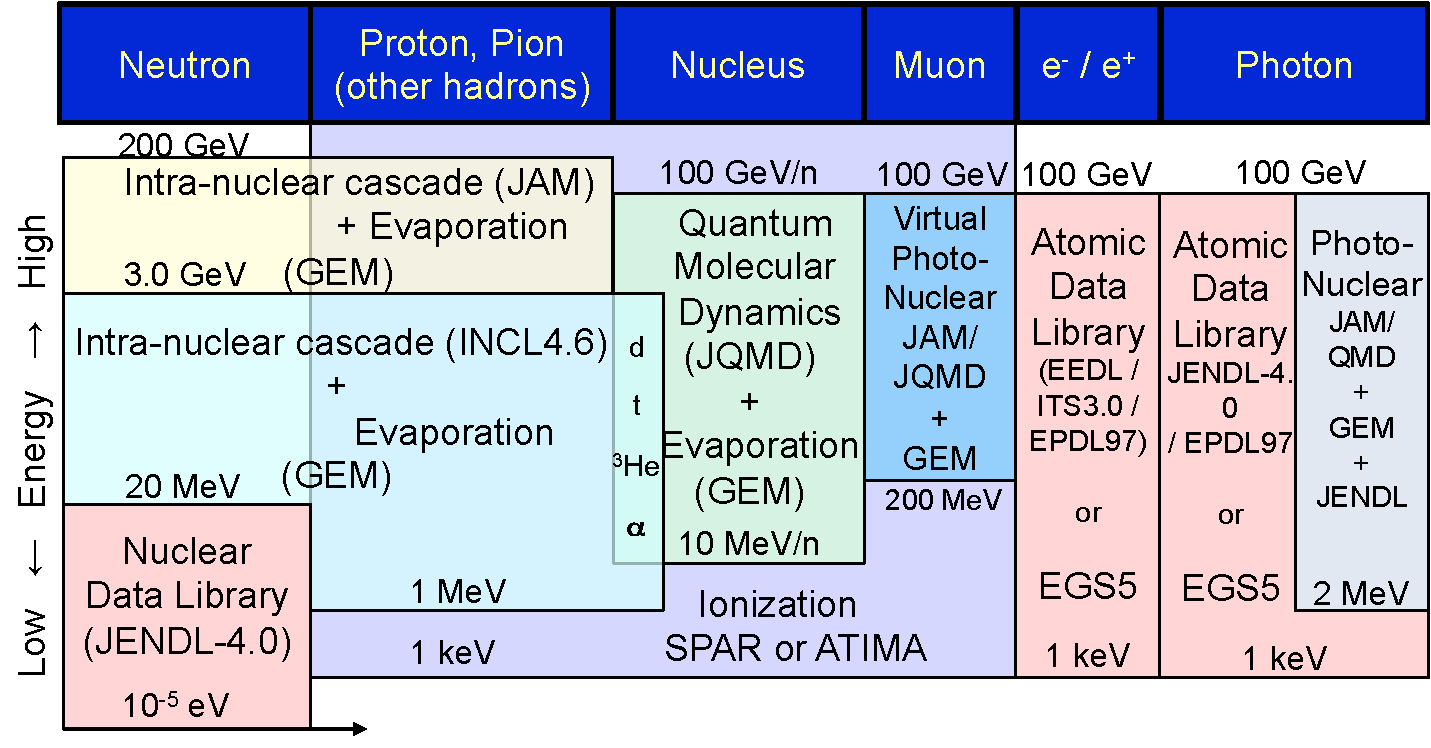
\includegraphics[scale=0.43]{chapter3/fig/physicalmodel.pdf}
 \caption{The physical model used in PHITS code. Default hadronic model is JAM\_INCL4.6\_JENDL, moreover, JAM\_BERT\_JENDL and JAM\_INC-ELF\_JENDL are able to be selected in PHITS code.}
 \label{phitsmodel}
\end{figure}
PHITS uses its own models for nuclear collisions and for hadron reactions.
The details of physical model in PHITS are shown in figure~\ref{phitsmodel}.
As for 8 GeV hadron collision, the Japanese nuclear library, JENDL-4.0, is employed in the low energy region ($\le$20 MeV).
Between 20 MeV and 3 GeV, there are three kinds of different model in hadron reaction, which are the INCL4.6~\cite{incl}, Bertini and INC-ELF~\cite{incelf}.

  \subsection{FLUKA}
~~~~~~FLUKA is a fully integrated particle physics Monte Carlo simulation package developed by CERN~\cite{fluka}.
Two hadronic models is included in FLUKA, the Generalized IntraNuclear Cascade (GINC) model in high energy region ($\ge$ 5 GeV) which is treated in the Glauber-Gribov formalism and PEANUT model in the low energy region~\cite{fluka2}.

  \subsection{GEANT4}
~~~~~~GEANT4 is the most powerful toolkit for simulation of high energy physics experiment~\cite{geant4}.
Like PHITS, GEANT4 is using the G4 neutron data library (G4NDL) in the energy less than 20 MeV.
Between 20 MeV and 5 GeV, three models, Binary, Bertini and INCL++, can be selected in G4.
G4 also provides the FTF String model from the range of 5 GeV to 20 TeV and QG String model to 100 TeV.
%\begin{table}[H]
% \centering
% \begin{tabular}{lcrr} \hline
%  Procss & MARS & GEANT4 & PHITS \\ \hline \hline
%  $\mu$ capture & Modified Fermi-Teller Law & None & CHIPS \\ \hline
%  $\pi$ capture & Modified Fermi-Teller Law & INCL 4.6 & QGSP\_BERT 4.0 \\ \hline
%  Radiative $\mu$ capture & & & CHIPS \\ \hline
%  Low energy hadron production & CEM95 & BERT, INCL4.6, INC-ELF & BERT\_HP \\ \hline
% \end{tabular}
%\end{table}

 \section{Modification of PHITS code}
~~~~~~Here, the modification of PHITS code will be introduced to achieve the realastic simualtion of COMET experiment.
The main optimization of PHITS code is listed as follows.
\begin{itemize}
 \setlength{\itemsep}{-5pt}
 \item Bridged PHITS and the accelerator simulation code TURTLE.
 \item Enable to read the external field map.
 \item The charged particle can be bended in user defined field.
 \item The output file from PHITS can be read into GEANT4 code.
 \item Enable to use the ROOT toolkit in PHITS.
\end{itemize}

 \subsection{Proton beam}
The proton beam source is simulated by the accelerator simulation code, called TURTLE in COMET experiment.
The simulation of TURTLE has been already shown in figure~\ref{beam}, and one bunch of the proton beam where locates in front of production target is gaussian distribution with size of 2 cm $\times$ 0.8 cm and momentum of 8.9 MeV/c.
PHITS can read the external file as the radiation source, but due to the different coordinate used in PHITS and TURTLE.
One script has been written to convert the coordinate and pretend the PHITS dump file to be read. 
The proton beam used in radiation estimation is TURTLE data for phase-I and gaussian beam for phase-II, respectively.
\begin{figure}[H]
 \centering
 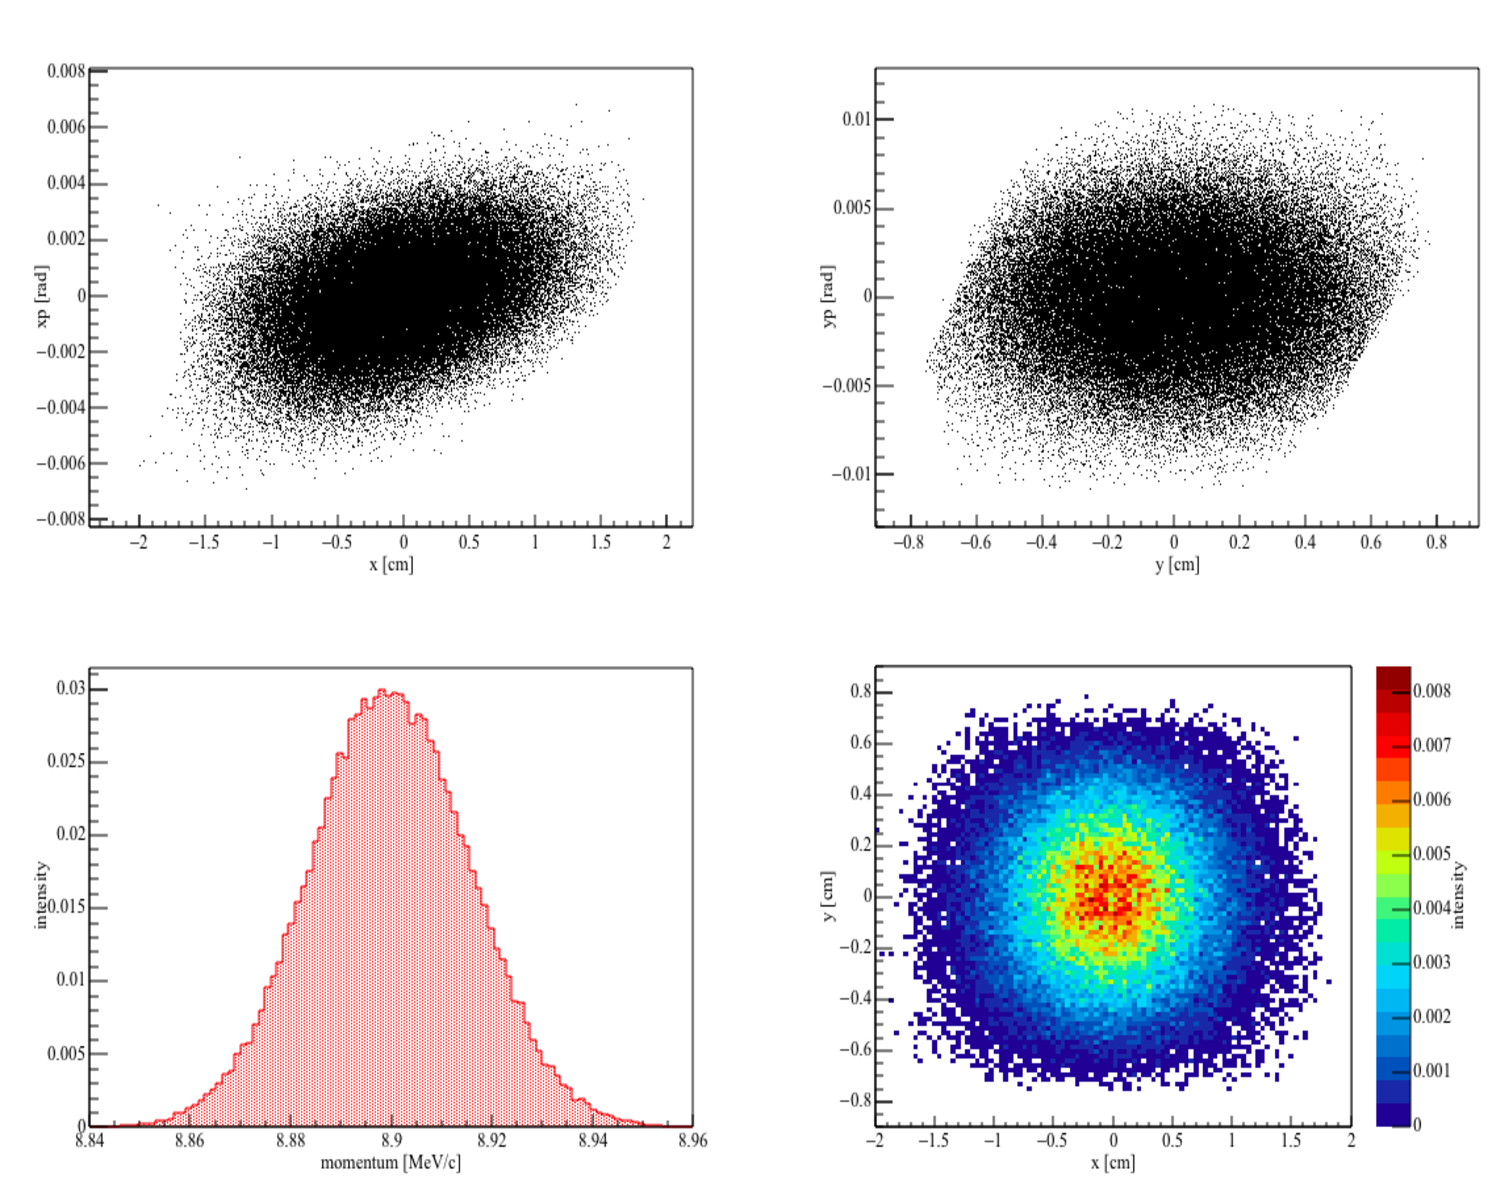
\includegraphics[scale=0.40]{chapter3/fig/beam.pdf}
 \caption{Proton beam distribution simulated by TURTLE code. Top two are the momentum distribution of x and y axis, respectively. Bottom two are the momentum distribution and spatial distribution. Here, intensity means the normalized intensity.}
 \label{beam}
\end{figure}
 
 \subsection{Magnetic field}
~~~~~~As for nowadays' PHITS, it still cannot bend the charged particles in user's field map.
However, the radiation estimation is affected by the magnetic field sensitively.
To solve this issue, one magnetic field interpolation subroutine written by C is compiled with FORTRAN files.
The details of the magnetic field interpolation is described in appendix A.
The charged particles are bended with a circular path in the magnetic field which is written as
\begin{equation}
 R = \frac{p}{eB} = \frac{m\gamma \beta c}{eB} = p \cdot \frac{3.336}{B}
\label{beq}
\end{equation}
To enesure the magnetic field interpolation, the uniform field map with 5 Tesla has been tested and the tracking is shown in~\ref{2uniform}.
Following the equation~\ref{beq}, the bending radius of 0.1 GeV/c momentum electron in 5 Tesla is 6.6 cm.
The radius from the simualtion is totally agree with the calculation.
 \begin{figure}[H]
  \centering
  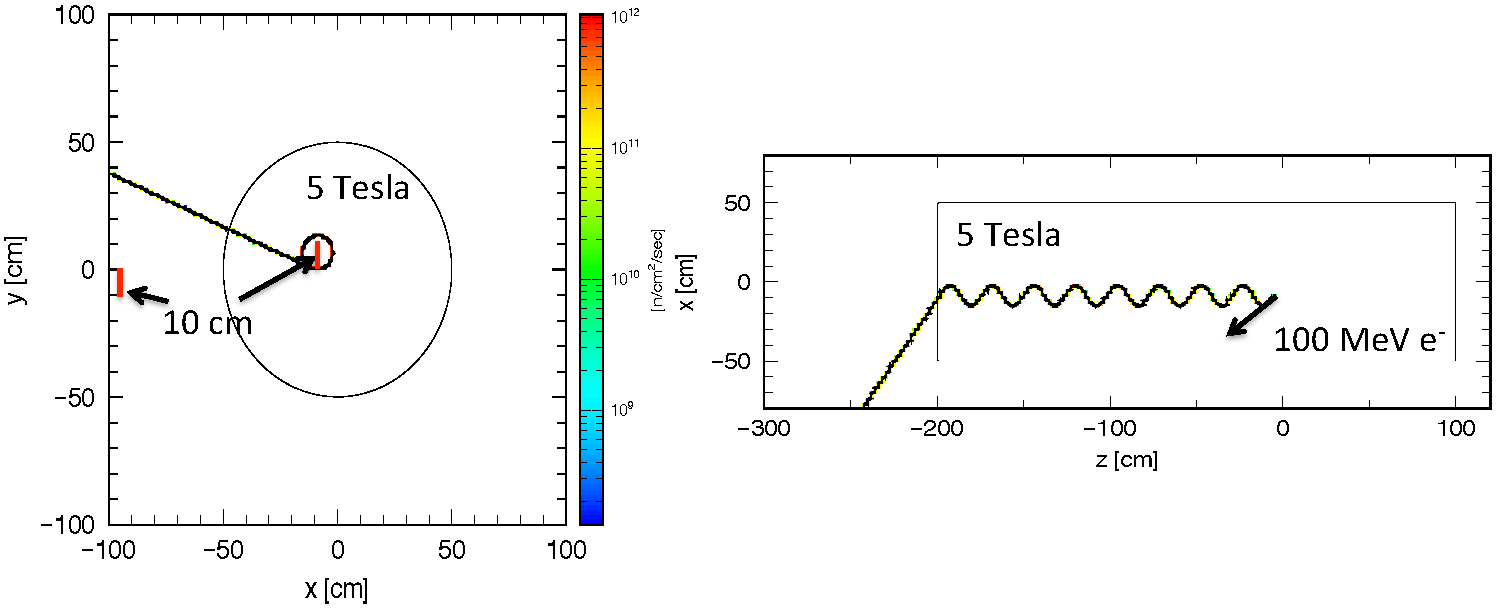
\includegraphics[scale=0.45]{chapter3/fig/magtest.pdf}
  \caption{Tracking of 100 MeV electron with uniform 5 Tesla field. One electron is injected with angle of 30 degree. Magnetic field is applied in a cylinder with radius of 50 cm and length of 300 cm.}
  \label{2uniform}
 \end{figure}
The field map included into COMET PHITS simulation is calculated by Finite Element Method (FEM) with iron yoke, which is shown in figure~\ref{field}.
There are still some missing part of field map, like the field around the iron yoke and proton beam transport pipe.
It will affect the proton beam transportation definitely, but this map is enough for the radiation study.

 \begin{figure}[H]
  \begin{subfigure}{0.3\textwidth}
   \centering
   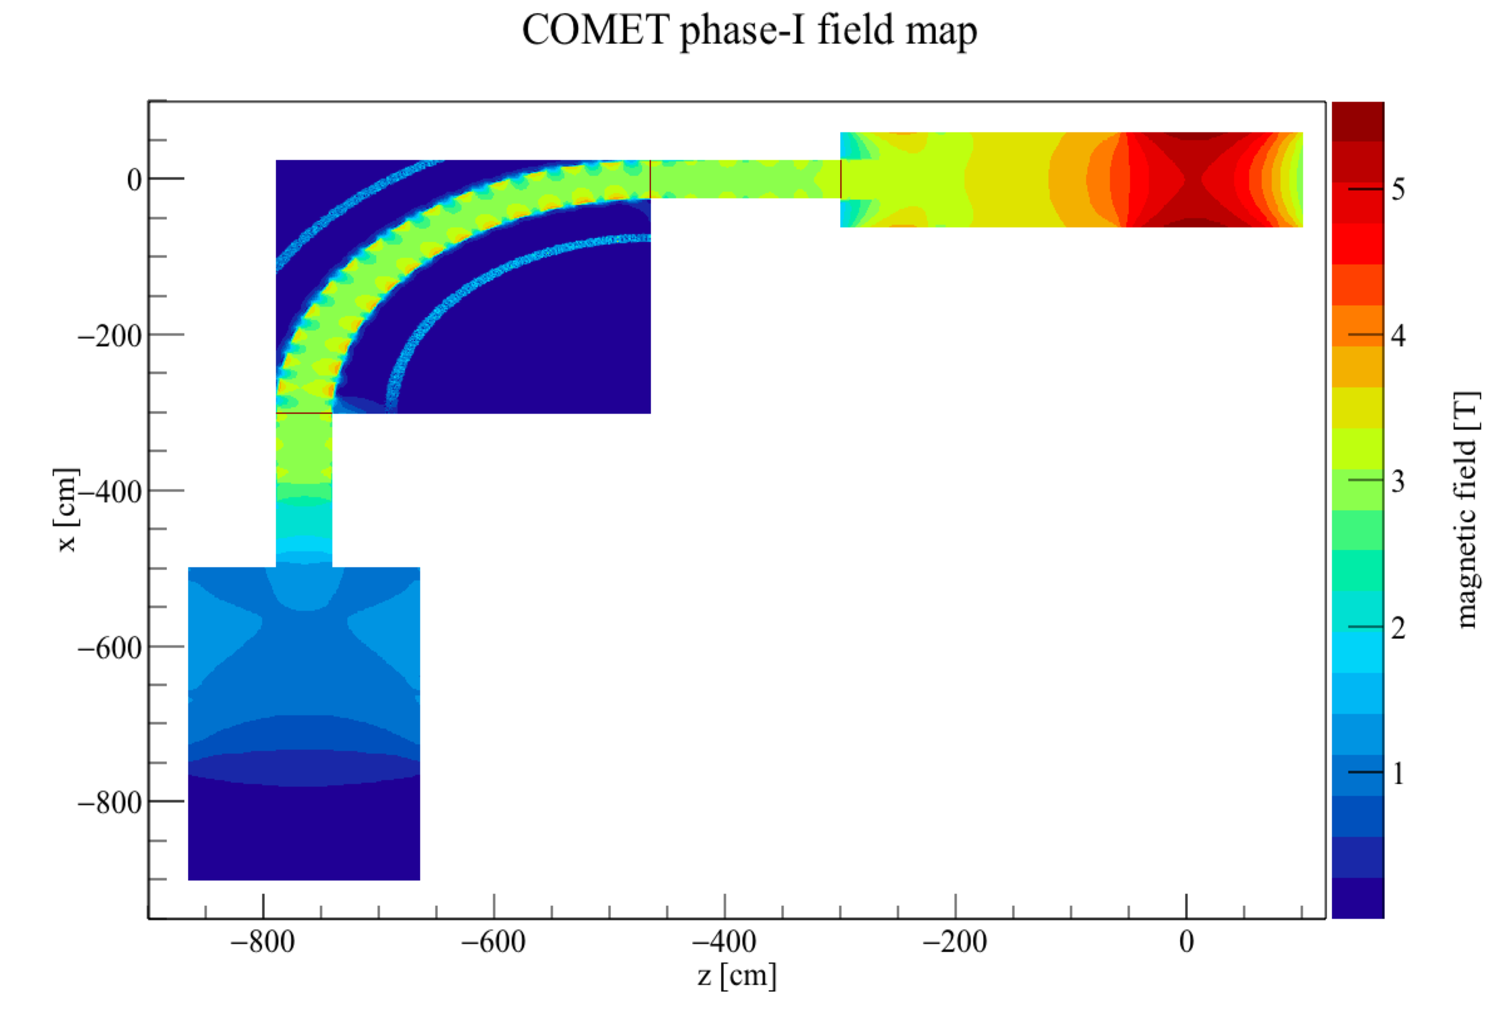
\includegraphics[scale=0.34]{chapter3/fig/fieldmap.pdf}
  \end{subfigure}
  \hspace{0.2\textwidth}
  \begin{subfigure}{0.3\textwidth}
   \centering
   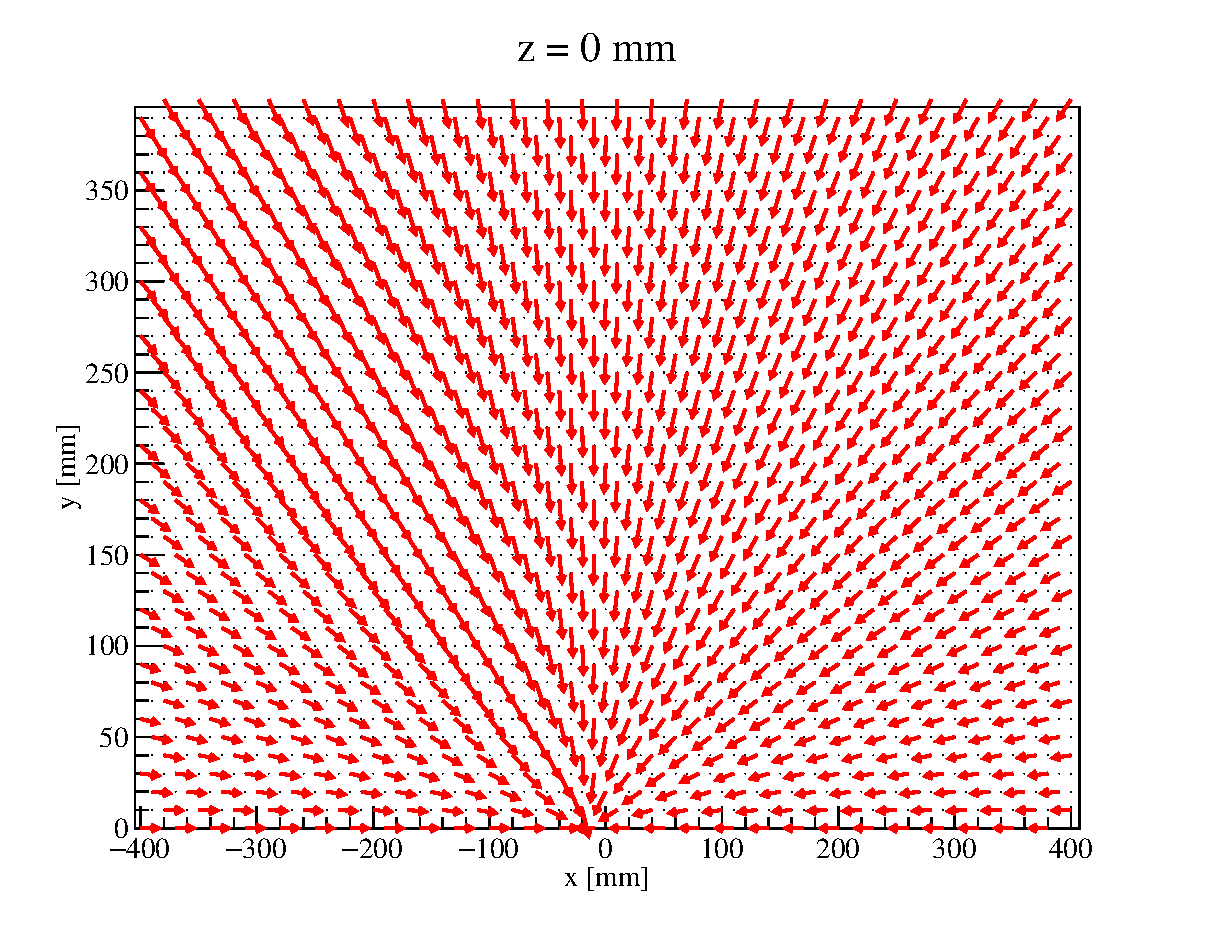
\includegraphics[scale=0.37]{chapter3/fig/fieldxy}
  \end{subfigure}
  \caption{Magnetic field map of phase-I experiment used in PHITS simulation. It is calculated by FEM with iron yoke. Mangetic field vector at z = 0 cm is shown on the right.}
  \label{field}
 \end{figure}

 \section{Prompt radiation}
  \subsection{Physical model comparison}
~~~~~~Since PHITS does not include a lot of physics model involved muon such as muon decay on the orbits, specific X-ray of muon capture, rate decay of muon et al., on the other hand, GEANT4 physics model is almost implement compared to PHITS, the comparison of particle yield between GEANT4 and PHITS is necessary to make sure the missing physics model can be neglected in radiation estimation.

The comparison is taken by using a very simple geometry, which is only one graphite target with 60 cm length and 2 cm radius.
Incident proton beam is 8 GeV with gaussian distribution.
Magnetic field is included in the region around target with 30 cm radius and 140 cm length.
As the result shown in figure~\ref{model} and table~\ref{2model}, the integral yield of pion and muon from target predicted by PHITS is higher than GENAT4's with factor 12.9\%.
For the neutron, the production yield has 17\% difference between GEANT4 and PHITS.
\begin{table}[H]
 \centering
 \begin{tabular}{cccccc} \hline \hline
  & $\mu^-$ [n/proton] & $\pi^-$ [n/proton] & $\mu^+$ [n/proton] & $\pi^+$ [n/proton] & neutron [n/proton] \\ \hline
  GEANT4 & 0.033 & 0.613 & 0.053 & 0.786 & 2.891 \\
  PHITS & 0.034 & 0.723 & 0.044 & 0.876 & 3.464 \\ \hline
  $\sigma$ & -3\% & -15\% & 21\% & -10\% & -17\% \\ \hline \hline
 \end{tabular}
 \caption{Comparison of PHITS with GEANT4. $\sigma$ represents (G4-PHITS)/PHITS.}
 \label{2model}
\end{table}
The backward production of muon and pion at high energy region is difficult to predict because of the lack of experimental data.
Especially for the COMET experiment which is employed the backward muon, prediction of backward muon and pion is quite different from the different physics model.
Thus, as the comparison of backward pion and muon at 1 m far from the target, compared with JAM\_BERT\_JENDL, the pion energy spectrum predicted by QGSP\_BERT\_G4NDL has high energy tail and lower peak.
Because the pion only comes from the high energy cascade model, the different must be between JAM and QGSP.
  \begin{figure}[H]
   \begin{subfigure}{0.3\textwidth}
    \centering
	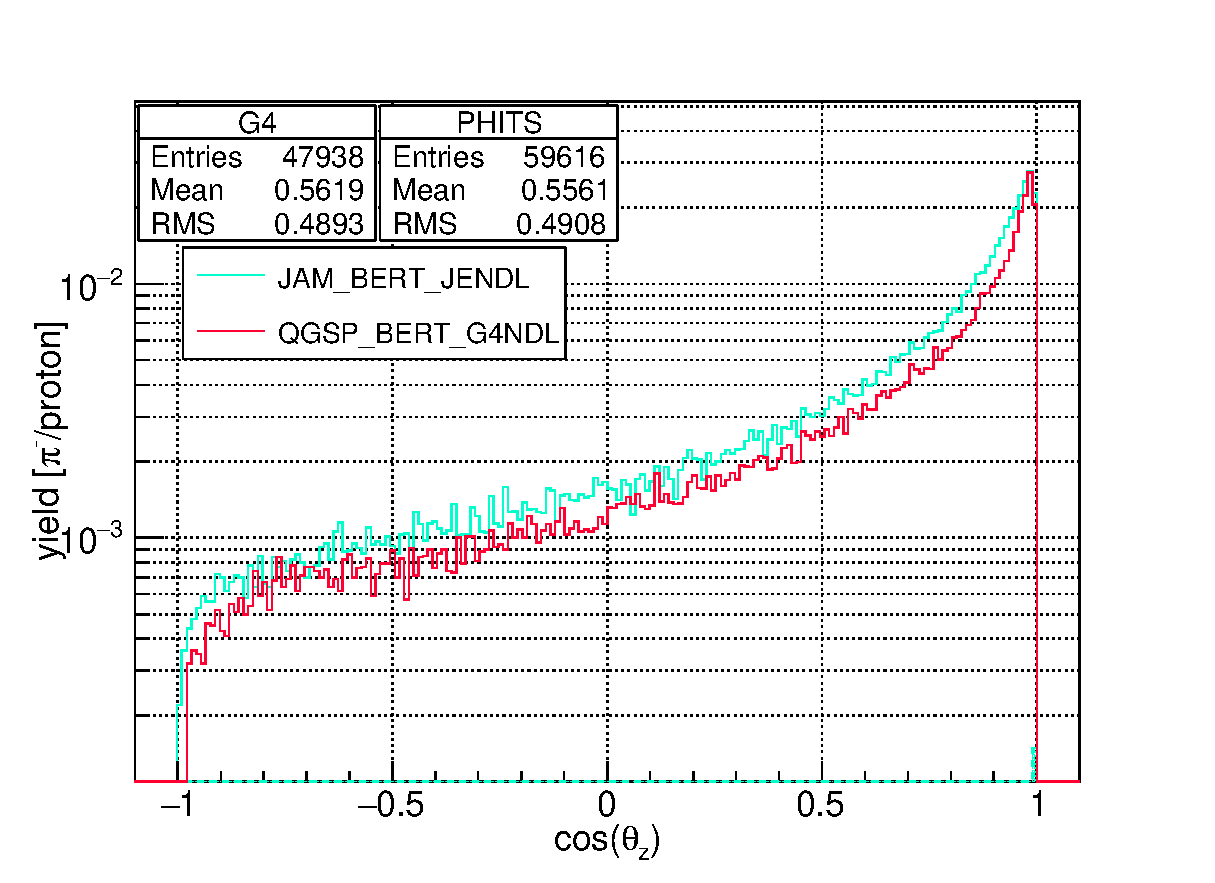
\includegraphics[scale=0.43]{chapter3/fig/backward}
   \end{subfigure}
   \hspace{0.2\textwidth}
   \begin{subfigure}{0.3\textwidth}
    \centering
	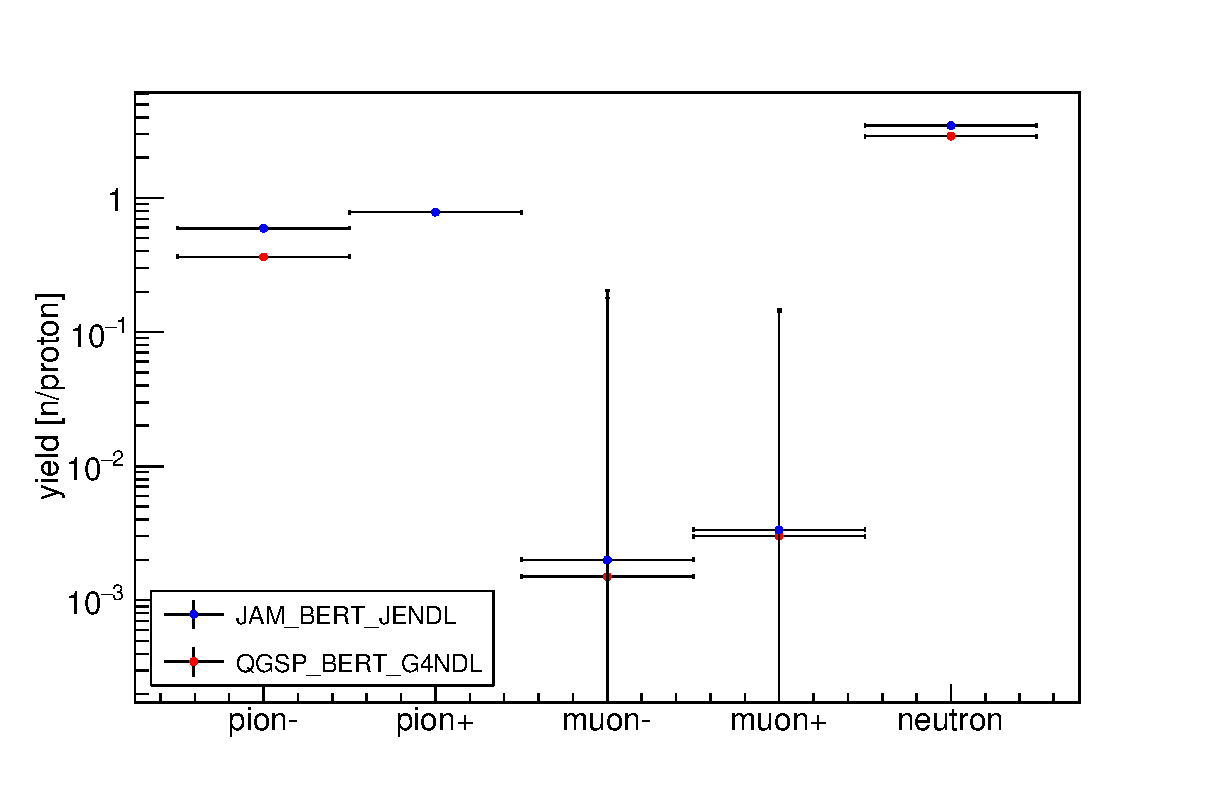
\includegraphics[scale=0.43]{chapter3/fig/production}
   \end{subfigure}
   \caption{Compared the backward particle yield and integral yield with GEANT4 and PHITS. Left one is the backward pion and muon yield, red and blue line represent the yield calculated by QGSP\_BERT\_G4NDL and JAM\_BERT\_JENDL respectively. Right one shows the integral yield of pion and muon from target, red and blue point are the result of QGSP\_BERT\_G4NDL and JAM\_BERT\_JENDL.}
   \label{model}
  \end{figure}

  \subsection{Geometry}
~~~~~~The geometry plays an important role in radiation simulation, especially for the high energy physics.
Every detail of COMET phase-I geometry is established in PHITS simulation in terms of the design drawing from KEK.
 \begin{figure}[H]
   \centering
   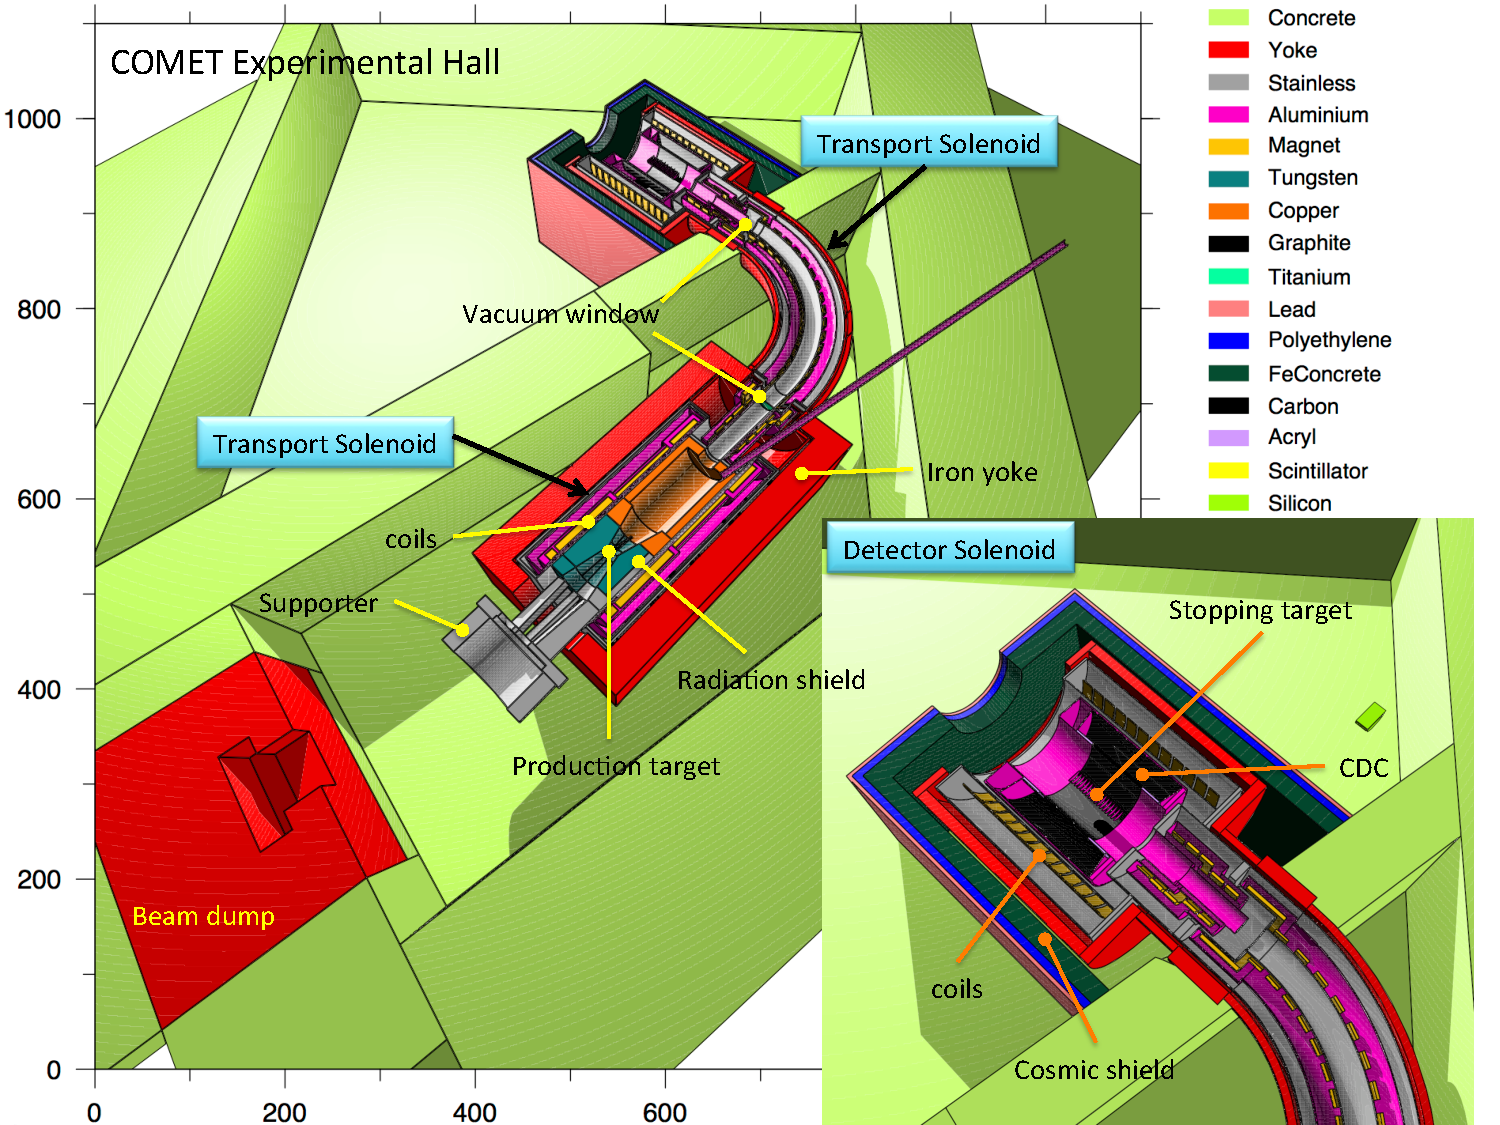
\includegraphics[scale=0.5]{chapter3/fig/geo.pdf}
   \caption{COMET phase-I experiment geometry in PHITS simulation.}
   \label{geom}
  \end{figure}
As shown in figure~\ref{geom}, the COMET experimental hall is seperated by concrete wall with 1 m thickness at end of 90 degree bending and 2 m at beam dump.
The concrete wall between experimental hall and control room and accelrator hall is with 3 m thickness to prevent the radiation leaking.
Beam dump consists of iron yoke with 1.5$\times$1.5$\times$1 m and 2.5$\times$2.5$\times$1 m holes which is same to the Mu2e beam absorber design and concrete~\cite{mu2ereport}.
Ceiling board is made of iron yoke with thickness of 0.6 m, gas (air) with thickness of 0.7 m and concrete with 3.7 m thickness.
Shielding supporter structure is made of stainless steel (SUS-304) with two holes for proton beam exit and target changing.
Radiation shield is employed the composit shield which will be described later.
In the muon beamline, two 1 mm titanium vacuum windows are set up in the end of pion capture solenoid and muon transport solenoid respectively.
Cosmic shield is consist of 20 cm concrete with 50\% iron, 10 cm polythylene and 10 cm lead.

  \subsection{Radiation estimation}
~~~~~~Since only backward pion is employed to create muon in high magnetic field, the main radiation is neutron and photon because they are not affected with magnetic field.
As implemented the geometry and magnetic field, the neutron and photon distribution is calculated and shown in figure~\ref{2photon}.
Because the geometry is only for phase-I experiment, the production target is replaced from graphite to pure tungsten target, and the proton beam intensity is changed to 4.4$\times$10$^{13}$ pps to estimate the radiation for phase-II experiment.
\begin{figure}[H]
   \begin{subfigure}{0.3\textwidth}
    \centering
    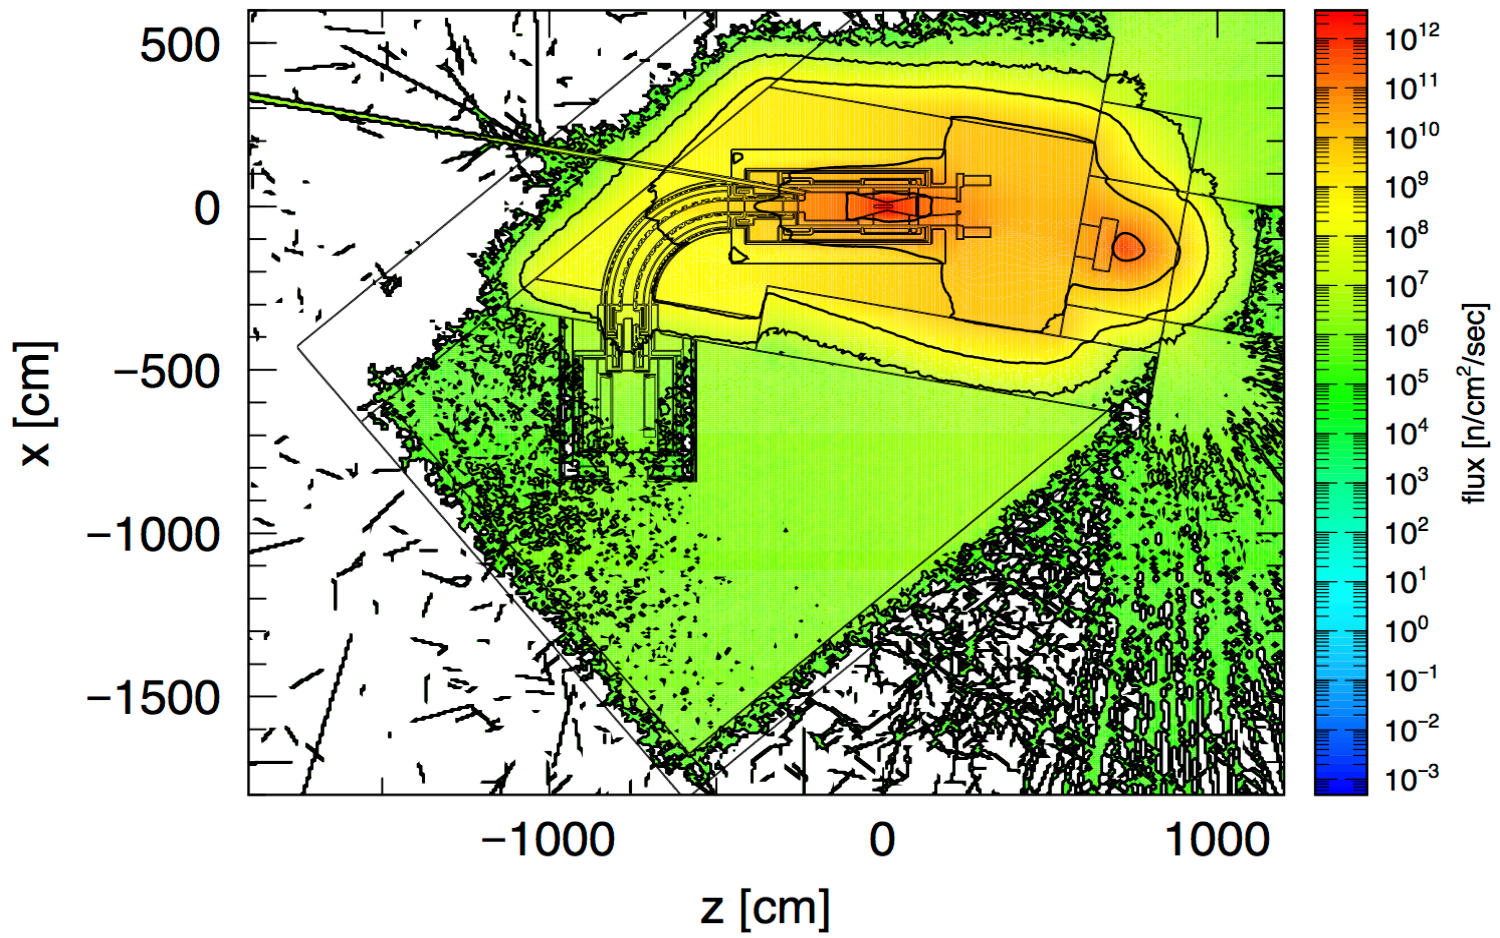
\includegraphics[scale=0.32]{chapter3/fig/neutronzx.pdf}
   \end{subfigure}
   \hspace{0.2\textwidth}
   \begin{subfigure}{0.3\textwidth}
    \centering
	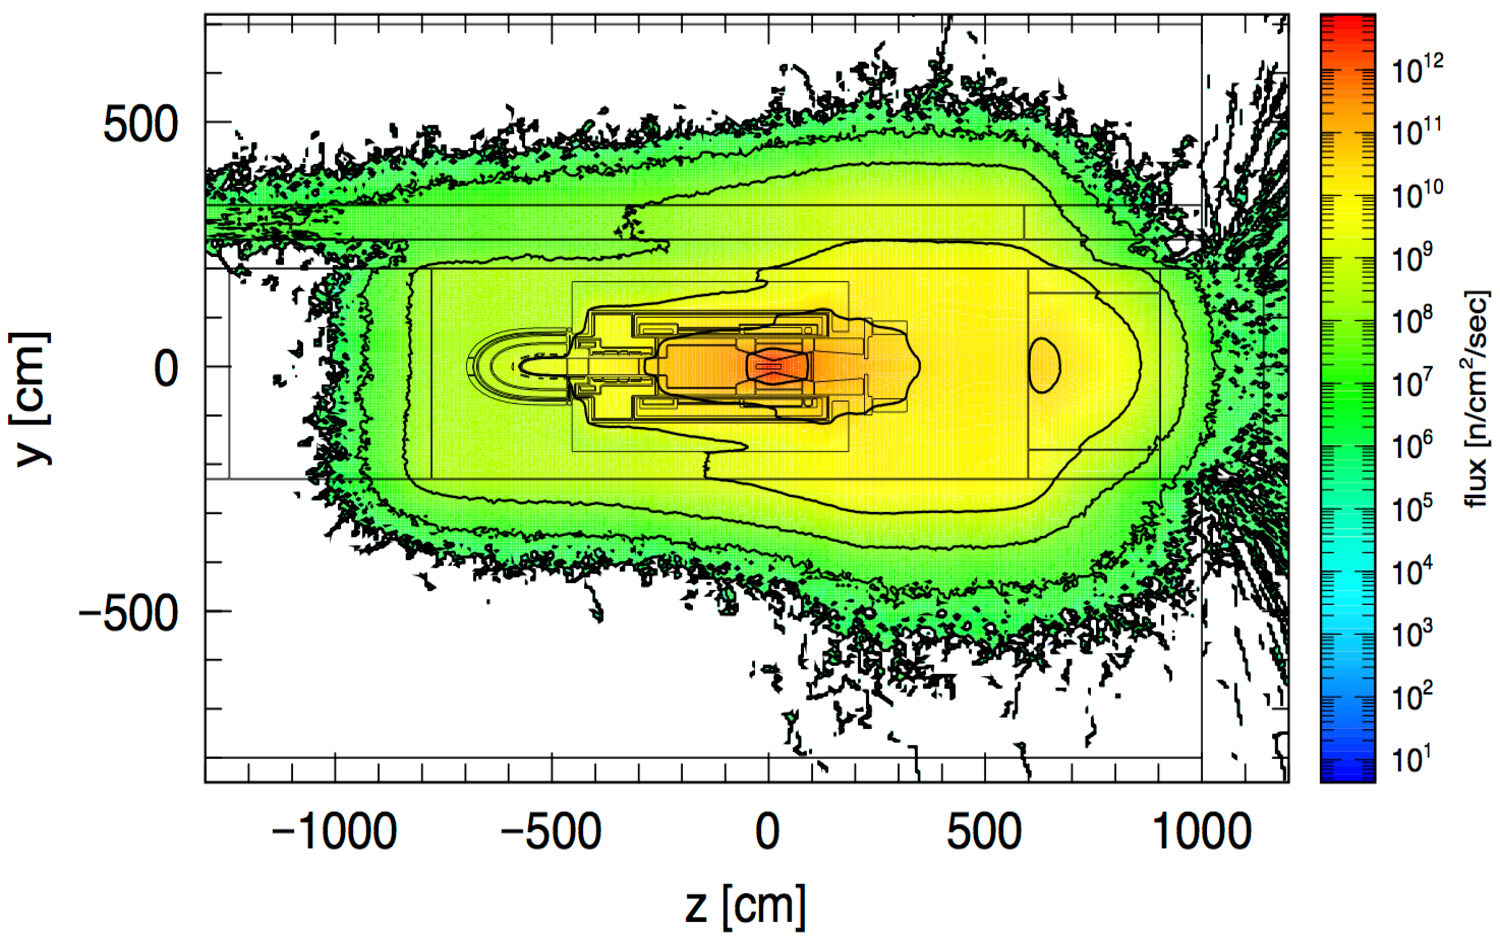
\includegraphics[scale=0.32]{chapter3/fig/neutronzy.pdf}
   \end{subfigure}
  % \caption{\it The phase-II neutron distribution calculated with phase-II target and beam intensity.}
  % \label{neutrondist}
  \end{figure}
  \begin{figure}[H]
   \begin{subfigure}{0.26\textwidth}
   \centering
   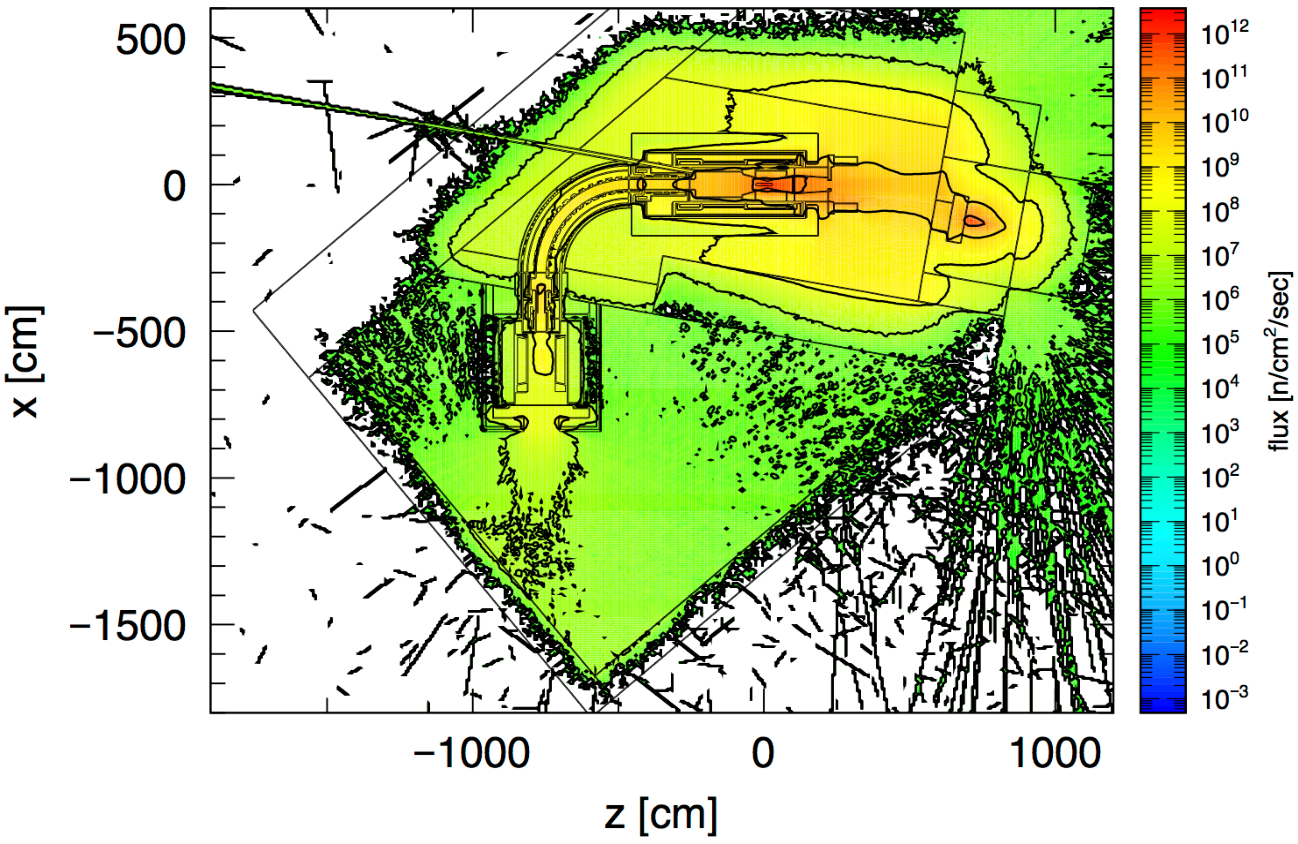
\includegraphics[scale=0.36]{chapter3/fig/photonzx.pdf}
   \end{subfigure}
   \hspace{0.2\textwidth}
   \begin{subfigure}{0.26\textwidth}
   \centering
   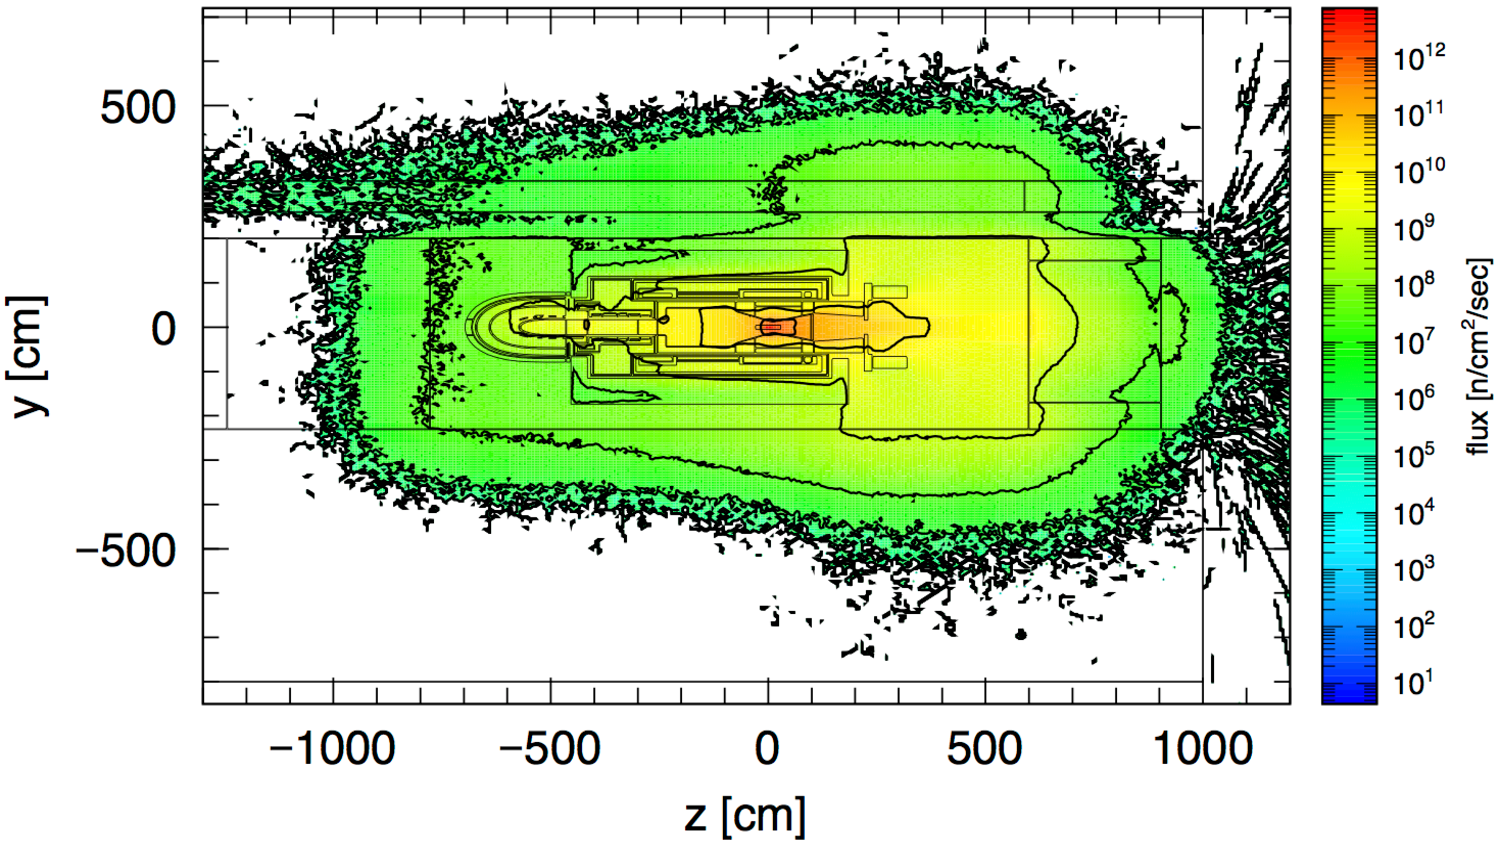
\includegraphics[scale=0.34]{chapter3/fig/photonyz.pdf}
   \end{subfigure}
   \caption{Neutron and photon distribution for COMET phase-II experiment. Top two show the neutron distribution from x-z and y-z view. Bottom two are the distribution of photon from x-z and y-z view.}
   \label{2photon}
  \end{figure}
Furthermore, to prevent neutrons leak to the detector room, the concrete wall with 2 m thick is replaced by iron yoke.
Even if the iron yoke is employed as a wall here, it still has 5$\times$10$^6$ n/cm$^2$/sec neutrons at least which leak from experimental room to detector room which is 5 times higher than phase-I exiperment.
The neutron along the muon beamline is with low energy and it is easy to be capture or scattered in the detector solenoid.
While, as for the photon, it comes from the neutron capture, muon capture, bremsstrahlung et al.
Thus, the photon in the detector solenoid is about 10$^9$ n/cm$^2$/sec at peak, which is 100 times higher than phase-I experiment at same place.

Figure~\ref{2bending} shows the energy spectrum of muon, photon and neutron for phase-II experiment at the end of 90 degree bending.
Compared with the other particle, neutron and photon is most dominated particle along the beamline.
Almost neutron is in the range of low energy, and photon is with energy from 0.01 MeV to 100 MeV.
  \begin{figure}[H]
   \centering
   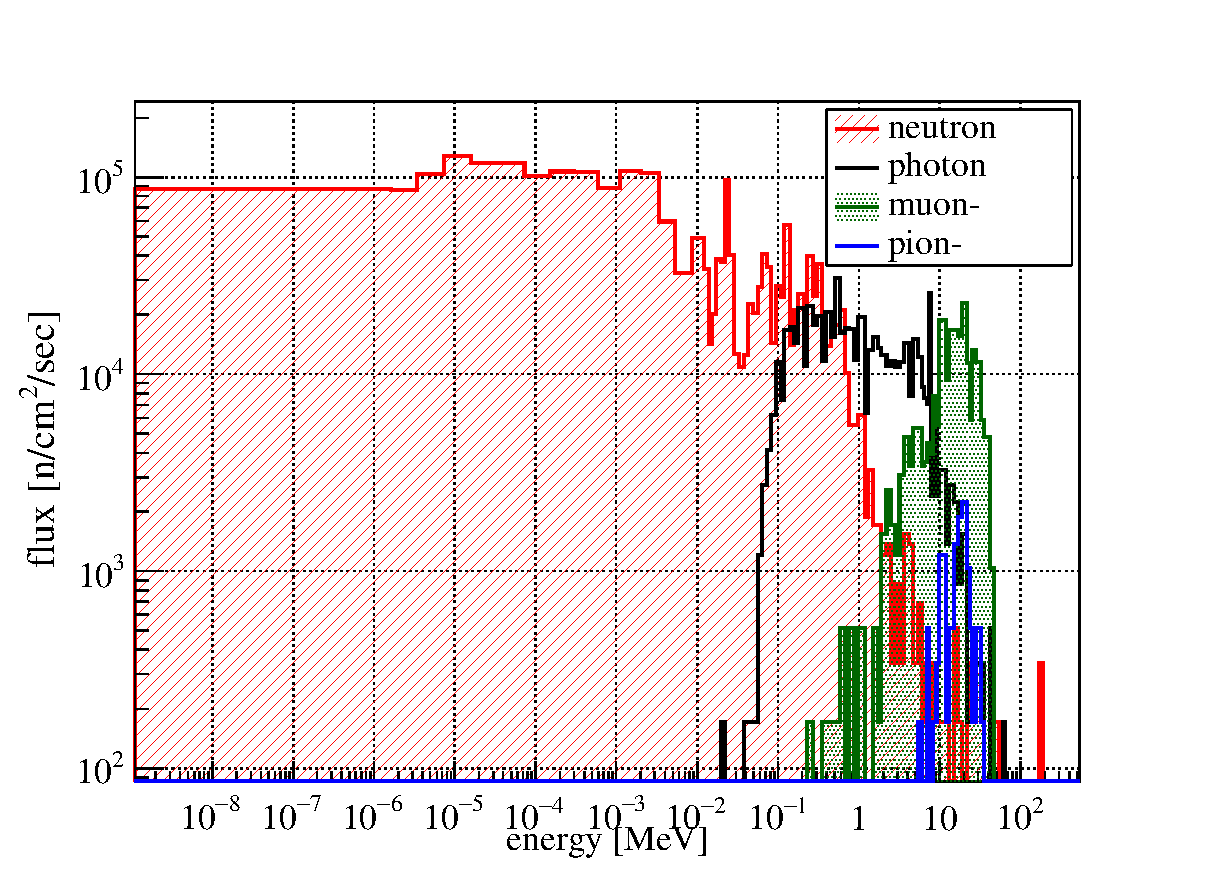
\includegraphics[scale=0.43]{chapter3/fig/Neutron}
   \caption{Energy spectrum of muon, photon and neutron from both experimental hall and beamline at the end of 90 degree bending. Most of neutrons are at the low energy region, and photon are all higher than 10 keV.}
   \label{2bending}
  \end{figure}
  \begin{figure}[H]
   \centering
   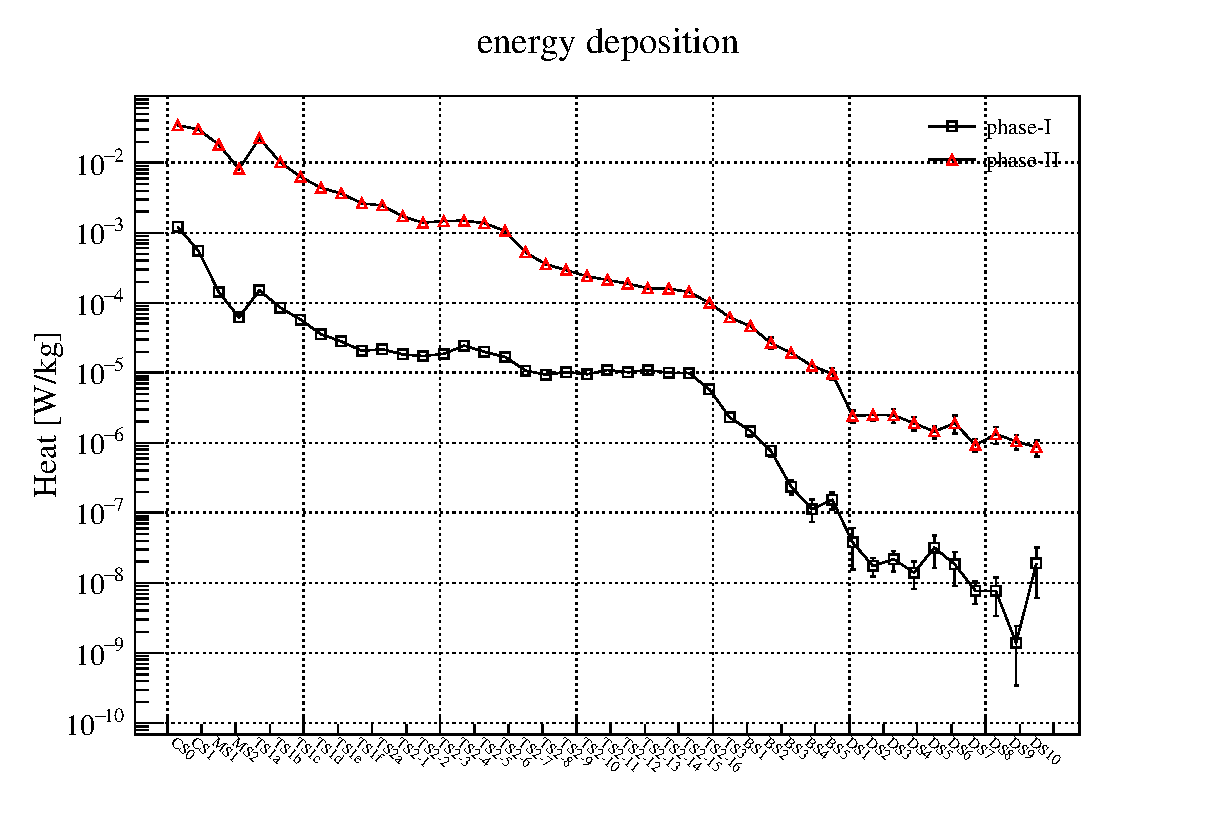
\includegraphics[scale=0.43]{chapter3/fig/heat}
   \caption{The energy deposition of each magnets in phase-I and phase-II experiment. Black and red point represent the energy deposition of phase-I and phase-II experiment respectively. The energy deposition of phase-II is one order higher than phase-I's, and its peak is located in CS0 coil.}
   \label{2heat}
  \end{figure}
The radiation remains thier energy into superconducting coils, which will cause the hot spot inside the magnets.
Once the hot spot is generated in the superconducting magnet, these magnets are at risk from quench.
The heat load of each magnet for phase-I and phase-II experiment are shown in figure~\ref{2heat}.
Compared with phase-I experiment, heat load of phase-II experiment is 10 times higher than phase-I experiment at least.
The peak of heat load is at CS0 coil which 0.03 W/kg correspending to 0.73 MGy for 280-day operation.

 \section{Residual radiation estimation}
~~~~~~To achieve the muon with higher intensity, the graphite target will be replaced by pure tungten target after phase-I experiment finished.
Thus, the residual radiation plays an important role in target changing and maintainance of the superconducting magnets.
The residual radiation has been investigated by using FLUKA code and PHITS code.

%  \subsection{Cross section comparison}
%~~~~~~In order to ensure the calculation of residual radiation, the activation cross section in PHITS code has been compared with the experimental data.
%Considering that COMET experiment is using the 8 GeV proton beam, which covers the INCL and JAM physical model in PHITS, the selection of the experimental data must be higher than 3.5 GeV.
%The activation cross section at high energy region has been compared with the experimental data from JASMIN collaboration~\cite{jasmin}.
%As the comparison shown in figure~\ref{yashima}, PHITS code has good agreement with the experimental data.
%\begin{figure}[H]
% \begin{subfigure}{0.3\textwidth}
%  \centering
%  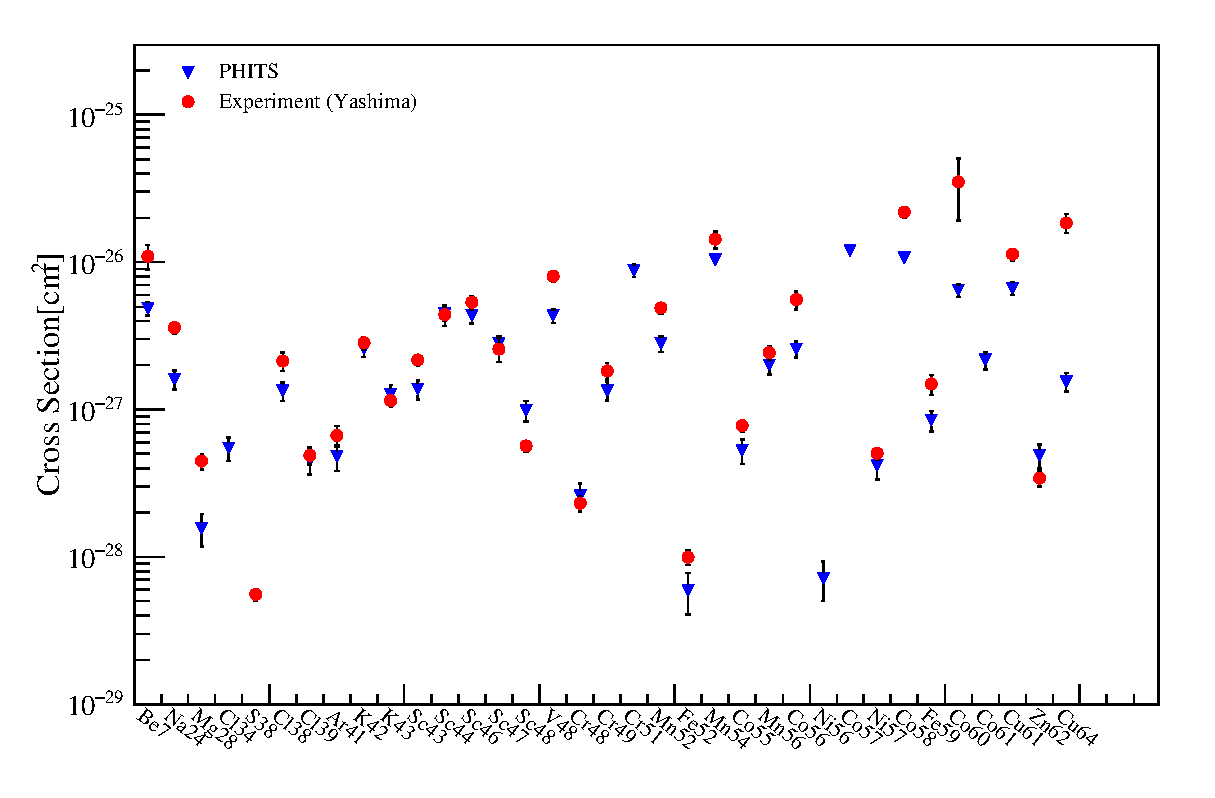
\includegraphics[scale=0.43]{chapter3/fig/copper}
  %\caption{\it Copper}
  %\label{fig:cuyashima}
%  \end{subfigure}
%  \hspace{0.2\textwidth}
% \begin{subfigure}{0.3\textwidth}
%  \centering
%  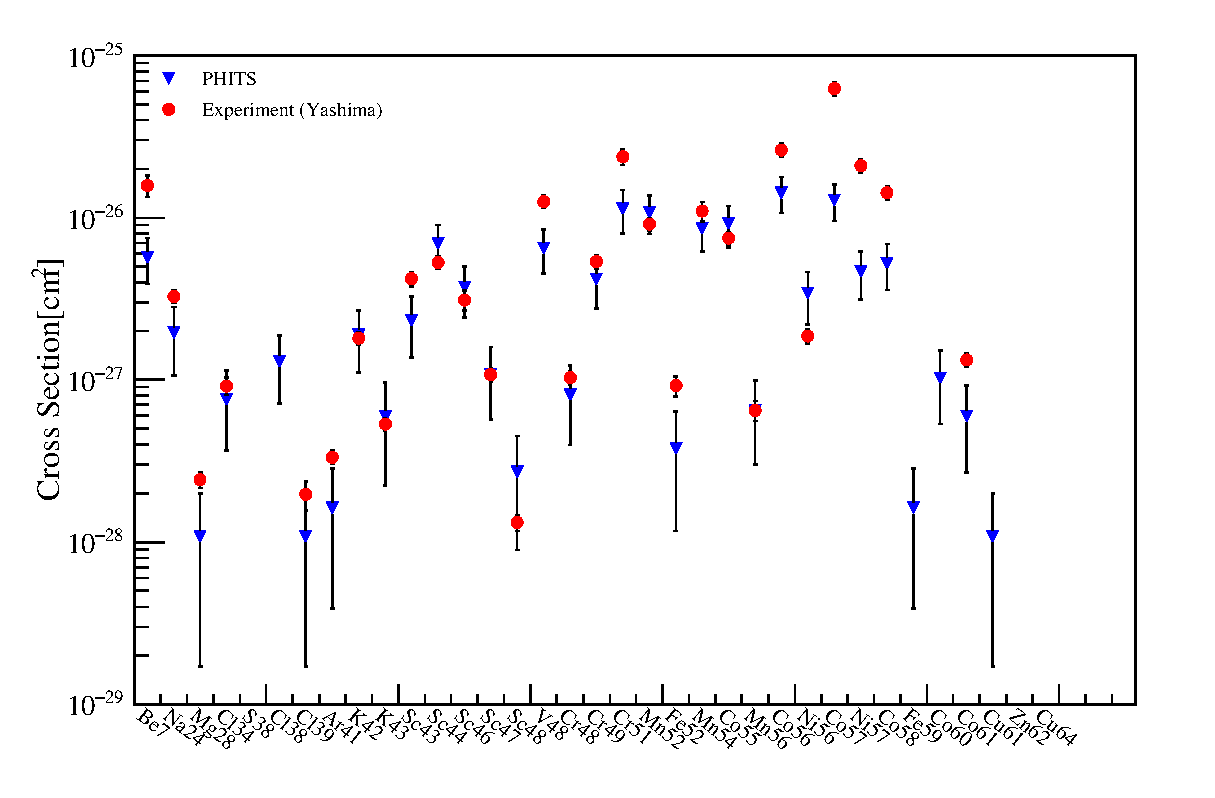
\includegraphics[scale=0.43]{chapter3/fig/nickel}
  %\caption{\it Nickel}
  %\label{fig:coyashima}
%  \end{subfigure}
%  \caption{Comparison of the activation cross section from experiment with PHTIS. Figure on left and right show the activation cross section of copper and nickel. The activation cross section is measured in FermiLAB by HPGe detector, using 120 GeV, 1.0$\times$10$^9$ pps roton beam.}
%  \label{yashima}
%\end{figure}

  \subsection{Residual radiation}
~~~~~~The residual radiation of each part of solenoid is estimated by PHITS and DCHAIN-SP code~\cite{dchain}.
DCHAIN-SP code is a dedicated software for the residual radiation developed by JAEA.
Using the result of nucleus yield from PHITS code, the photon flux and its intensity is able to be calculated by DCHAIN-SP.
Then, the distribution of residual radiation is estimated by
\begin{equation}
 E(\epsilon) = f(\epsilon) \cdot \phi(\epsilon)
\end{equation}
where $E(\epsilon)$ and $\phi(\epsilon)$ are the effective dose and the gamma ray flux calculated in DCHAIN-SP.
The fluence-to-effective dose conversion coefficients $f(\epsilon)$ is shown in reference~\cite{flco} with unit of Sv/cm$^2$.

The operation time schedule used in calculation are 1-year cooling after 1-month running with intensity of 2.5$\times$10$^{12}$ pps, which are all base on the phase-I experiment.
Residual radiation of vacuum vessel, magnet, radiation shield and iron yoke are given by figure~\ref{2part}.
To reduce the residual radiation as much as possible, considering copper is hard to weld with stainless steel, some parts of vacuum vessel is able to be changed to iron.
As listed in table~\ref{vecuum}, residual radiation of stainless steel is 10 times higher than iron's.
\begin{table}[H]
 \centering
 \begin{tabular}{ccc} \hline \hline
  & Stainless steel & Iron  \\ \hline
  Radiation dose [$\mu$Sv/h] & 7.00 & 0.65 \\ \hline \hline
 \end{tabular}
 \caption{Residual radiation of vacuum vessel between CS0 and iron yoke.}
 \label{vecuum}
\end{table}
Thus, the stainless steel is replaced by iron for vacuum vessel outside the superconducting magnet due to magnetism of iron.
 \begin{figure}[H]
  \centering
  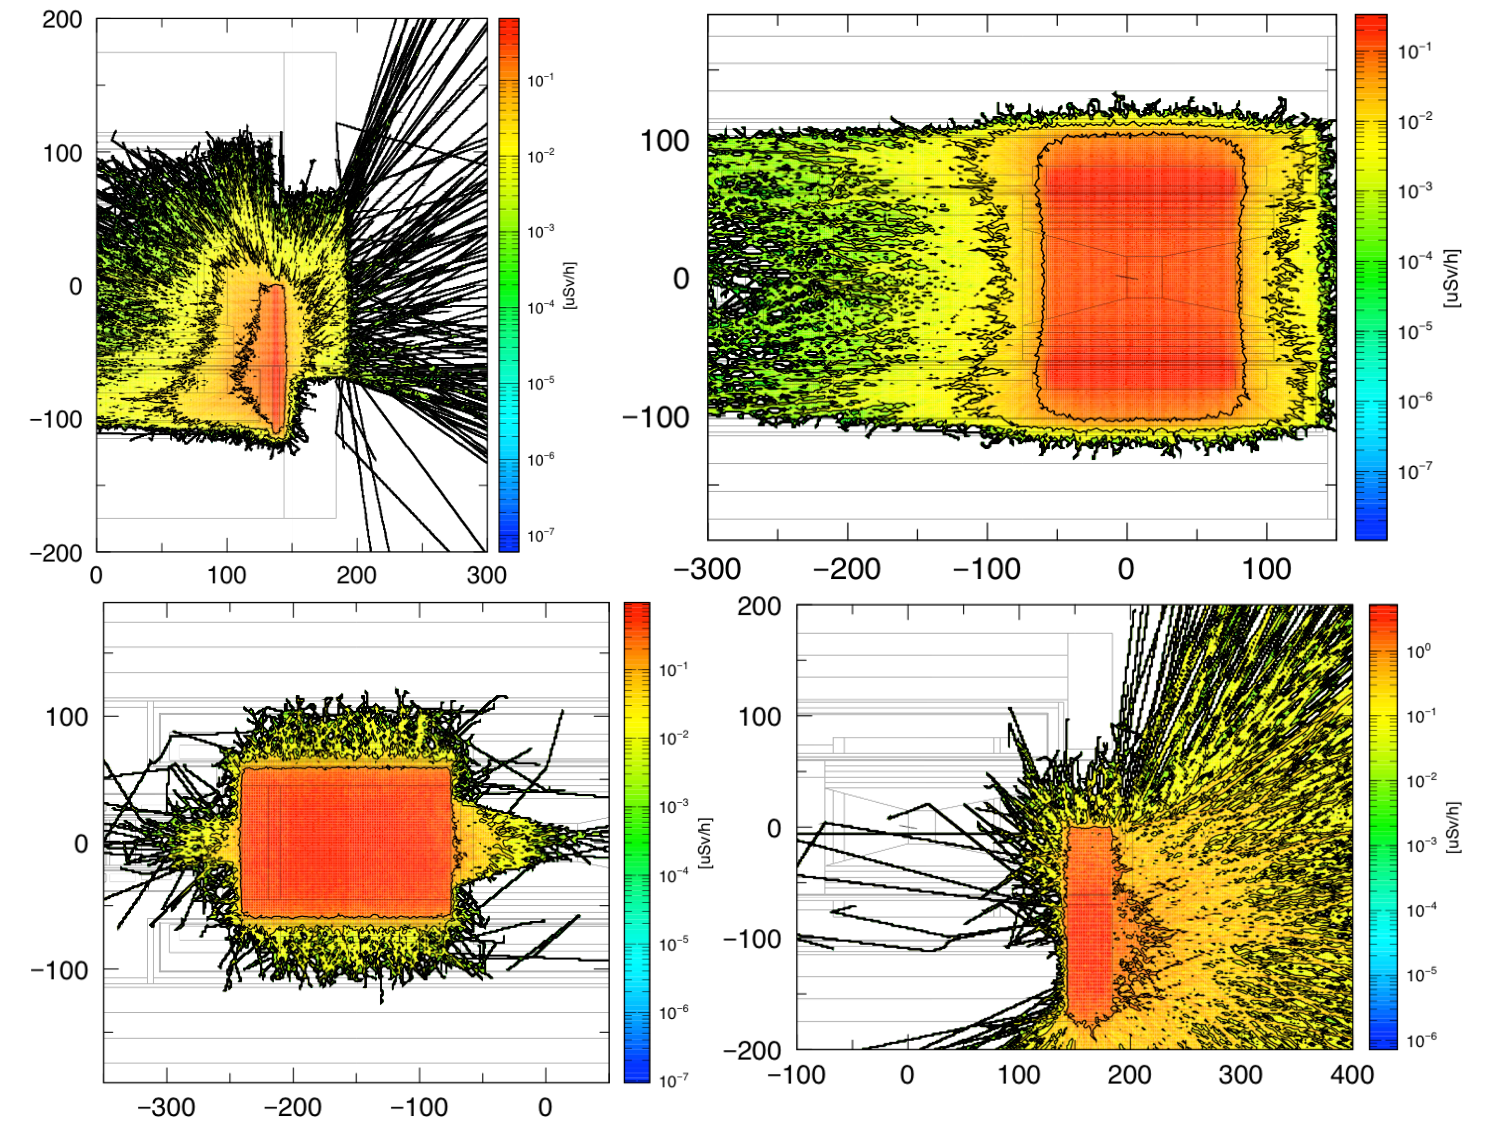
\includegraphics[scale=0.43]{chapter3/fig/partres.pdf}
  \caption{Residual radiation of vacuum vessel, magnet, radiation shield and iron yoke with 1 month operation and 10 month cooling.}
  \label{2part}
 \end{figure}
The residual radiation of superconducting magnet is calculated as one conductor which consists of aluminum, copper and NbTi with density of 4.0 g/cm$^3$.
The activity and radiation dose given by figure~\ref{2dose} shows that the maximum radiation dose is 0.33 $\mu$Sv/h after 1 month operation and 10 month cooling for phase-I experiment and the peak of activation is at CS0 and CS1.
Isotopes like $^{93}$Nb, $^{22}$Na, $^3$H, $^{60}$Co et al. with long half life are generated in CS1 and CS0 coils.
 \begin{figure}[H]
  \begin{subfigure}{0.3\textwidth}
   \centering
   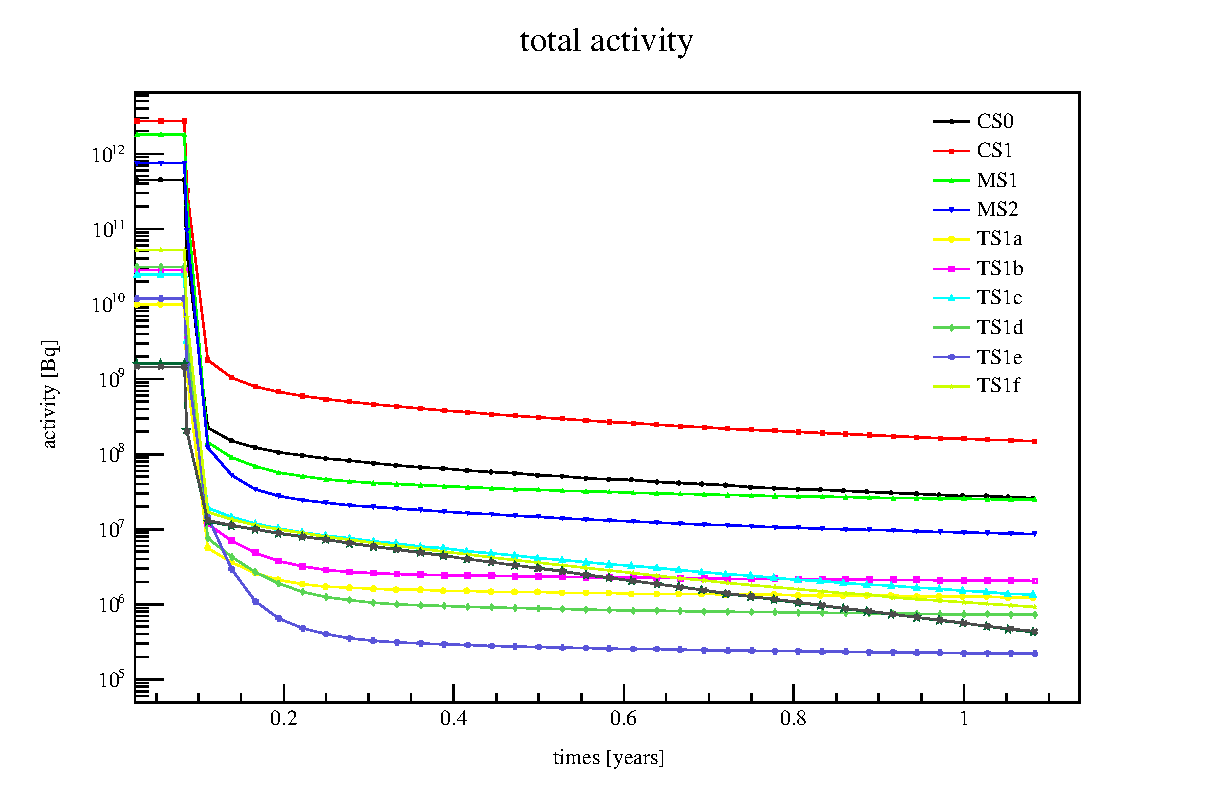
\includegraphics[scale=0.45]{chapter3/fig/activity.eps}
  \end{subfigure}
  \hspace{0.2\textwidth}
  \begin{subfigure}{0.3\textwidth}
   \centering
   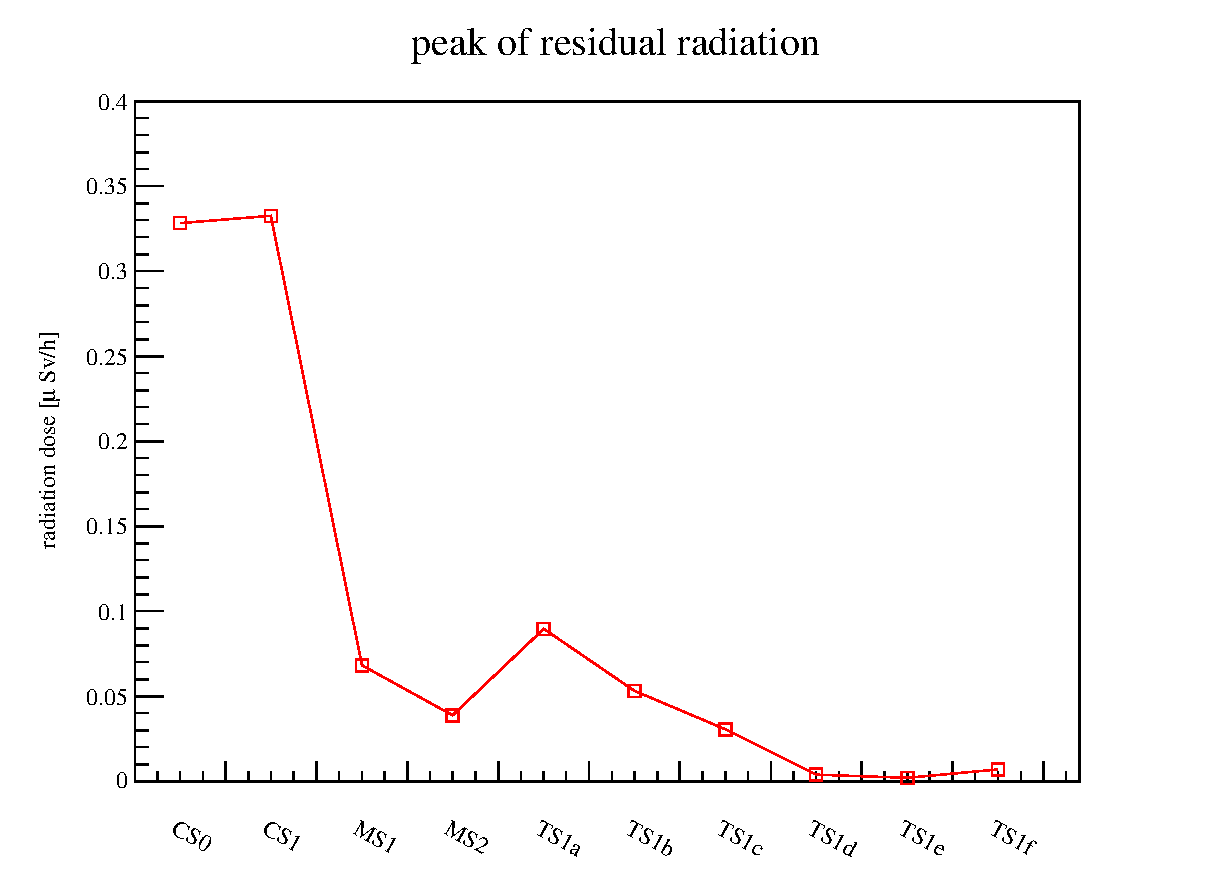
\includegraphics[scale=0.40]{chapter3/fig/dose.eps}
  \end{subfigure}
  \caption{Activity and peak of dose equivalent of each magnets with 1-month operation and 10-month cooling.}
  \label{2dose}
 \end{figure}

Because PHITS and DCHAIN-SP only can calculate the residual radiation from a defined region, it may cause the average of the radiation if the geometry is cut to many tiny meshes.
Figure~\ref{2dose2} (left) shows the total dose equivalent predicted by PHITS and DCHAIN-SP.
It is added from many parts of small regions.
The maximum dose equivalent is predicted to 0.75 mSv/h for 1-month operation and 10-month cooling at production target.
To ensure the dose equivalent, we also compare this result with FLUKA code which can simulate the residual radiation dose without region cutting.
M. Brugger et al. present the residual radiation calculated from FLUKA code has good agreement experimental data~\cite{brugger}.
As the result shown in figure~\ref{2dose2} (right), the maximum dose equivalent is predicted to 3.74 mSv/h with same time schedule, which is 5 times higher than PHITS result.
In figure~\ref{dosepo}, the dose equivalent at different position along the axis is compared.
Besides the place where peak is, the dose equivalent is quite similar between the FLUKA and PHITS.
Difference may be owing to the mesh cutting of PHITS calculation around target.
 \begin{figure}[H]
  \begin{subfigure}{0.3\textwidth}
   \centering
   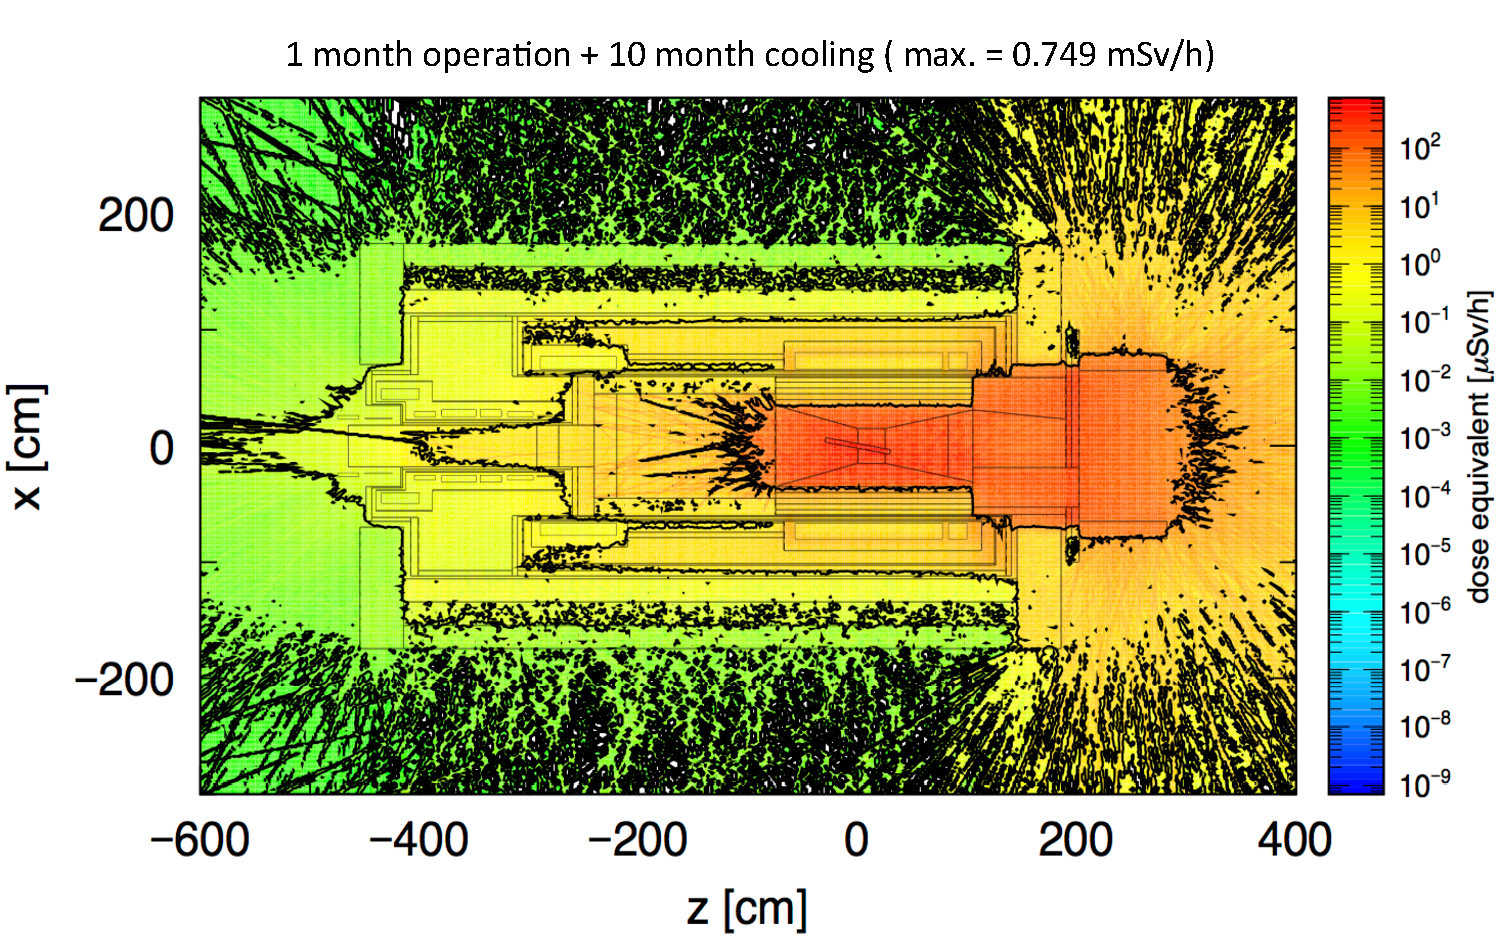
\includegraphics[scale=0.33]{chapter3/fig/phitsdose.pdf}
  \end{subfigure}
  \hspace{0.2\textwidth}
  \begin{subfigure}{0.3\textwidth}
   \centering
   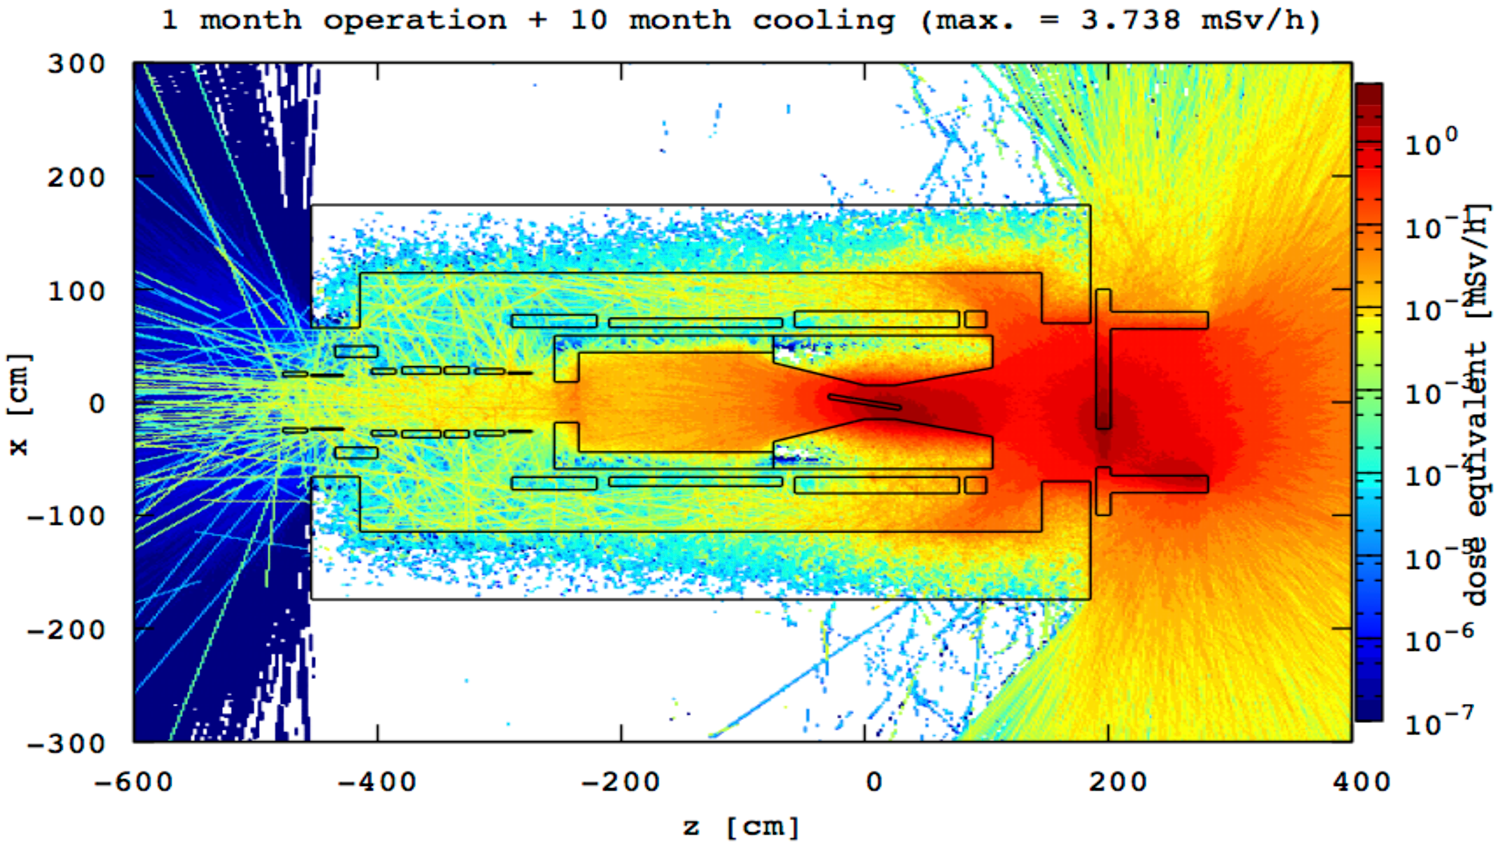
\includegraphics[scale=0.33]{chapter3/fig/flukadose.pdf}
  \end{subfigure}
  \caption{Compared the residual radiation distribution of pion capture solenoid between PHITS and FLUKA. Left and right represent the PHITS and FLUKA result respectively.}
  \label{2dose2}
 \end{figure}
\begin{table}[H]
 \centering
 \begin{tabular}{ccccc} \hline \hline
  Code & z = 0 & z = 300 & z = -300 & z = -500 \\
   & [mSv/h] & [mSv/h] & [mSv/h] & [mSv/h] \\ \hline
  FLUKA & 3.74 & 0.04 & 0.009 & 0.002 \\
  PHITS & 0.75 & 0.03 & 0.01 & 0.002 \\ \hline \hline
 \end{tabular}
 \caption{Compared the residual radiation along the z axis. z=0 is at the production target, z=-300 is 3 m far from the target on upstream of target, z=300 is 3 m far from the target on dreamstream of target, and z=-500 is 5 m far from teh target.}
 \label{dosepo}
\end{table}
Because of the target changing after phase-I experiment, this residual radiation is still too high for co-workers.
Table~\ref{2time} gives the maximum residual radiation after cooling for 10 months, 1.75 year and 2 years.
\begin{table}[H]
 \centering
 \begin{tabular}{cc} \hline \hline
  Time [year] & Maximum residual radiation [mSv/h] \\ \hline
  0.83 & 3.738 \\
  1.75 & 1.125 \\
  2.00 & 1.013 \\ \hline \hline
 \end{tabular}
 \caption{Maximum residual radiation after cooling for 10 months, 1.75 year and 2 years.}
 \label{2time}
\end{table}
From this estimation, the residual radiation will be reduced about 3 times after cooling for 2 years compared with 10 month cooling.
Considering the beam dump is not included into this simulation, working for 1 hour is possible for co-workers.

 \section{Radiation shielding optimization}
~~~~~~The heat and radiation shield (HRS) is located around the production target to protect the superconducting from the radiation exposure.
This radiation shield consists of two parts, one is for protecting MS magnets, another one is for protecting CS magnets.
It is unable to take long time to change the radiation shield after phase-I experiment due to the residual radiation.
Thus, radiation shield must be designed for both phase-I and phase-II experiment.

Pure tungsten is most ideal material as the radiation shield due to its high density.
However, it has several disadvantages such as high costs, heavy mass and complex fabrication.
Therefore, some parts of radiation shield can be replaced by the other materials.

 \subsection{Radiation shield for MS}
~~~~~~Inside the superconducting magnets, radiation shield must be made of material without magnetism.
Thus, there are two candidates for MS radiation shield, copper and stainless steel.
The heat load of each CS and MS magnet when the copper and stainless steel is used as radiation is estimated by PHITS code in table~\ref{hrsload}.
It shows that copper shield has better shielding ability than stainless steel shield.
 \begin{table}[H]
 \centering
 \begin{tabular}{cccccc} \hline \hline
  & CS0 [W] & CS1 [W] & MS1 [W] & MS2 [W] & CS + MS [W] \\ \hline
  SUS304 & 8.03 & 51.82 & 27.80 & 10.49 & 98.13 \\
  Copper & 7.56 & 50.14 & 22.99 & 8.73 & 89.42 \\ \hline \hline
 \end{tabular}
 \caption{Heat load of stainless steel and copper shield.}
 \label{hrsload}
\end{table}
Considering the residual radiation of radiation shield, the actived isotopes and activity after 1-month operation and 10-month cooling are investigated and shown in table~\ref{2atom}.
Apparently, copper shield's activity is quite lower than stainless steel shield's.
Furthermore, the dose equivalent of copper and stainless steel shield are 1.51 $\mu$Sv/h and 7.02 $\mu$Sv/h respectively.

From the aspect of shielding ability and residual radiation, copper is the better material for MS radiation shield.
Noting that the induced current will be generated by the changing of magnetic field, the copper should be cut in somewhere.
\begin{table}[H]
 \centering
 \begin{tabular}{c}
  \begin{minipage}{0.4\textwidth}
  \centering
  \begin{tabular}{ccc} \hline \hline
   Nuclei & Activity [MBq] & Half life [year] \\ \hline
   $^{60}$Co & 192 & 5.27 \\
   $^{57}$Co & 111 & 0.75 \\
   $^{63}$Ni & 80.9 & 100 \\
   $^{58}$Co & 56.9 & 0.19 \\
   $^{54}$Mn & 54.7 & 0.86 \\
   $^3$H & 30.9 & 12.3 \\
   $^{55}$Fe & 29.3 & 2.73 \\
   $^{49}$V & 16.7 & 0.90 \\
   $^{56}$Co & 5.52 & 0.21 \\
   $^{65}$Zn & 5.13 & 0.67 \\ \hline \hline
  \end{tabular}
  %\caption{Actived isotopes of copper shield.}
  \end{minipage}
  \hspace{0.1\textwidth}
  \begin{minipage}{0.4\textwidth}
  \centering
  \begin{tabular}{ccc} \hline \hline
   Nuclei & Activity [MBq] & Half life [year] \\ \hline
   $^{55}$Fe & 4950 & 2.73 \\
   $^{54}$Mn & 1500 & 0.86 \\
   $^{49}$V & 878 & 0.90 \\
   $^{57}$Co & 585 & 0.75 \\
   $^{58}$Co & 387 & 0.19 \\
   $^{51}$Cr & 92.6 & 0.08 \\
   $^{59}$Fe & 29.4 & 0.12 \\
   $^{63}$Ni & 26.5 & 100 \\
   $^3$H & 26.0 & 12.3 \\
   $^{60}$Co & 21.7 & 5.27 \\ \hline \hline
  \end{tabular}
  %\caption{Actived isotopes of stainless steel shield.}
  \end{minipage}
 \end{tabular}
 \caption{Actived isotopes of copper (left) and stainless steel (right).}
 \label{2atom}
\end{table}

\subsection{Radiation shield for CS}
~~~~~~Proton is injected into pion capture solenoid with 10 degree, thus, a hot spot is created on the one side of CS1 and CS0 coils, which is the one of the reason why quench occurs.
Thus, the radiation shield for CS requires
\begin{itemize}
 \setlength{\itemsep}{-5pt}
 \item Limit the maximum heat load in coils.
 \item Limit the maximum radiation induced damage in coils.
 \item Reduce the mass of radiation shield.
 \item Pion yield should not be reduced significantly.
\end{itemize}

To eliminate the hot spot and keep the balance, the low radiation region which corresponds to the side far to incident proton enables to be fabricated by another kind of material.
As for the material, the ideal material is pure tungsten but only the tungsten alloy is cheaper and easy to fabricate.
Thus, the details of tungsten alloy (AN-1800) are list in table~\ref{alloy}.
 \begin{figure}[H]
  \begin{subfigure}{0.3\textwidth}
   \centering
   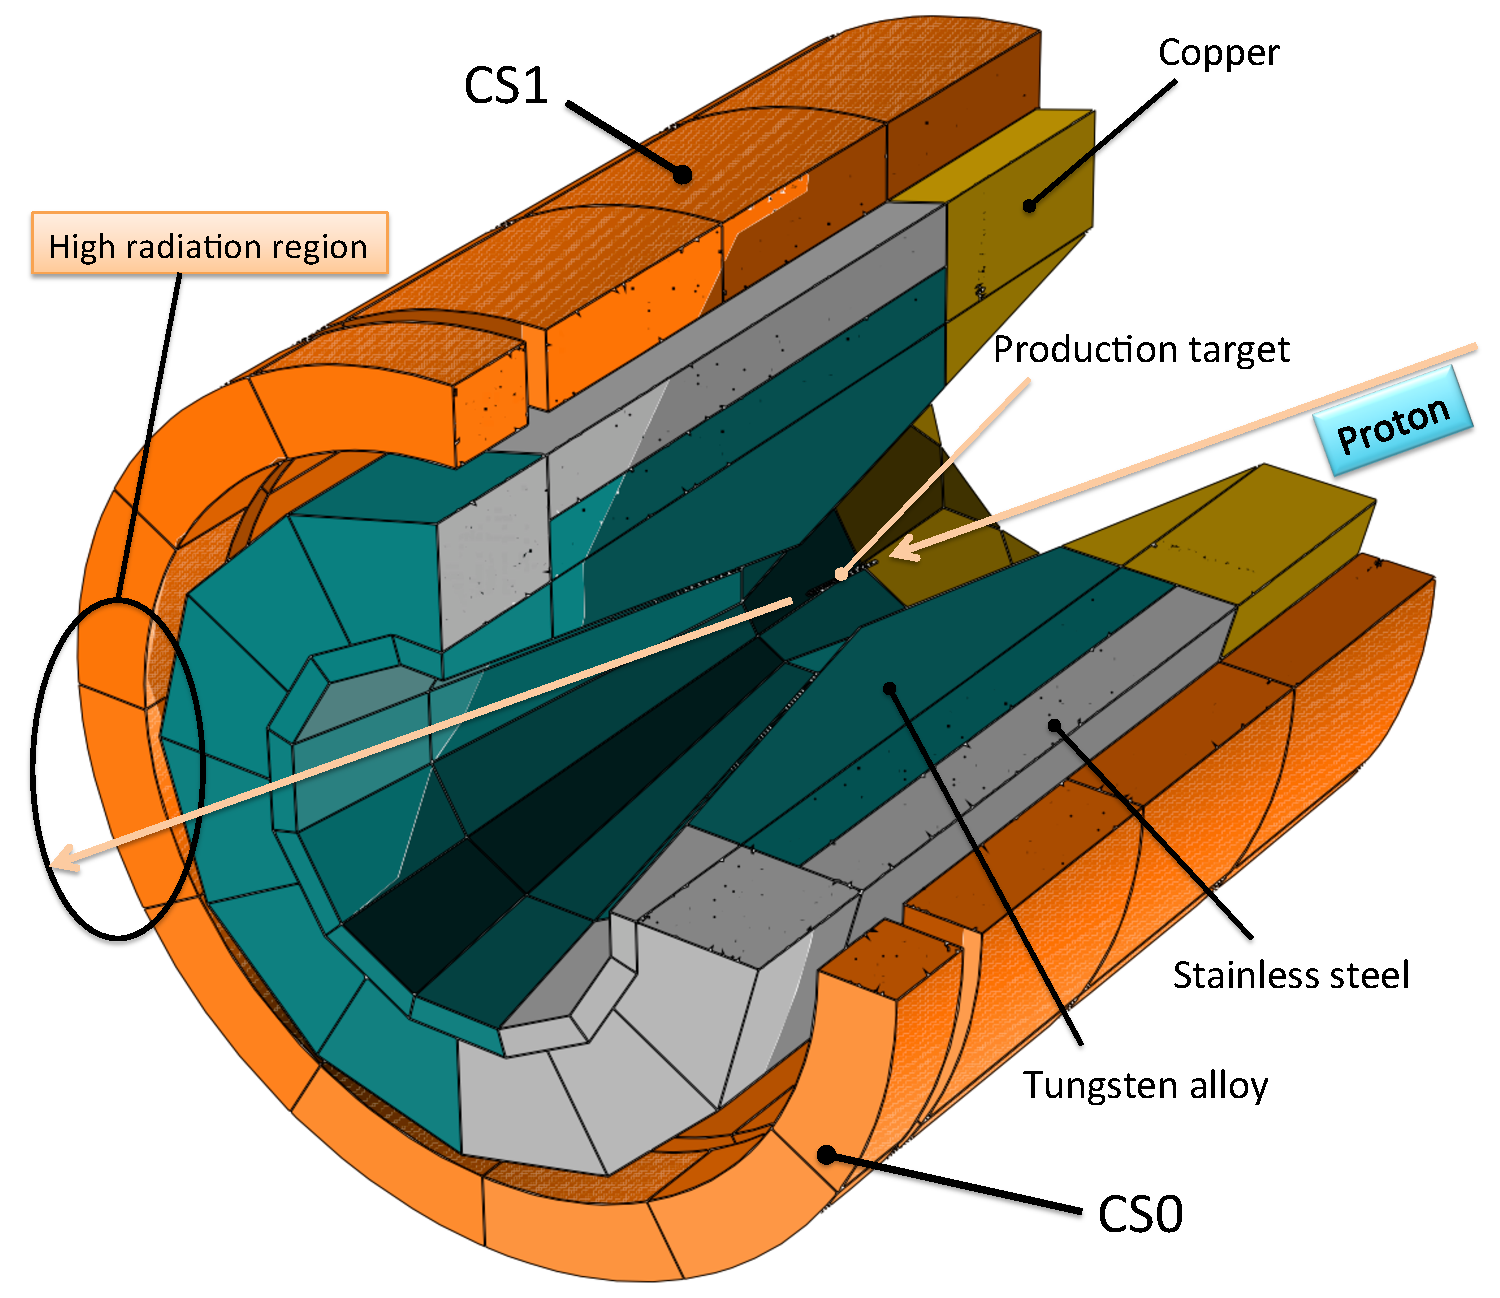
\includegraphics[scale=0.3]{chapter3/fig/shielding.pdf}
  \end{subfigure}
  \hspace{0.2\textwidth}
  \begin{subfigure}{0.3\textwidth}
   \centering
   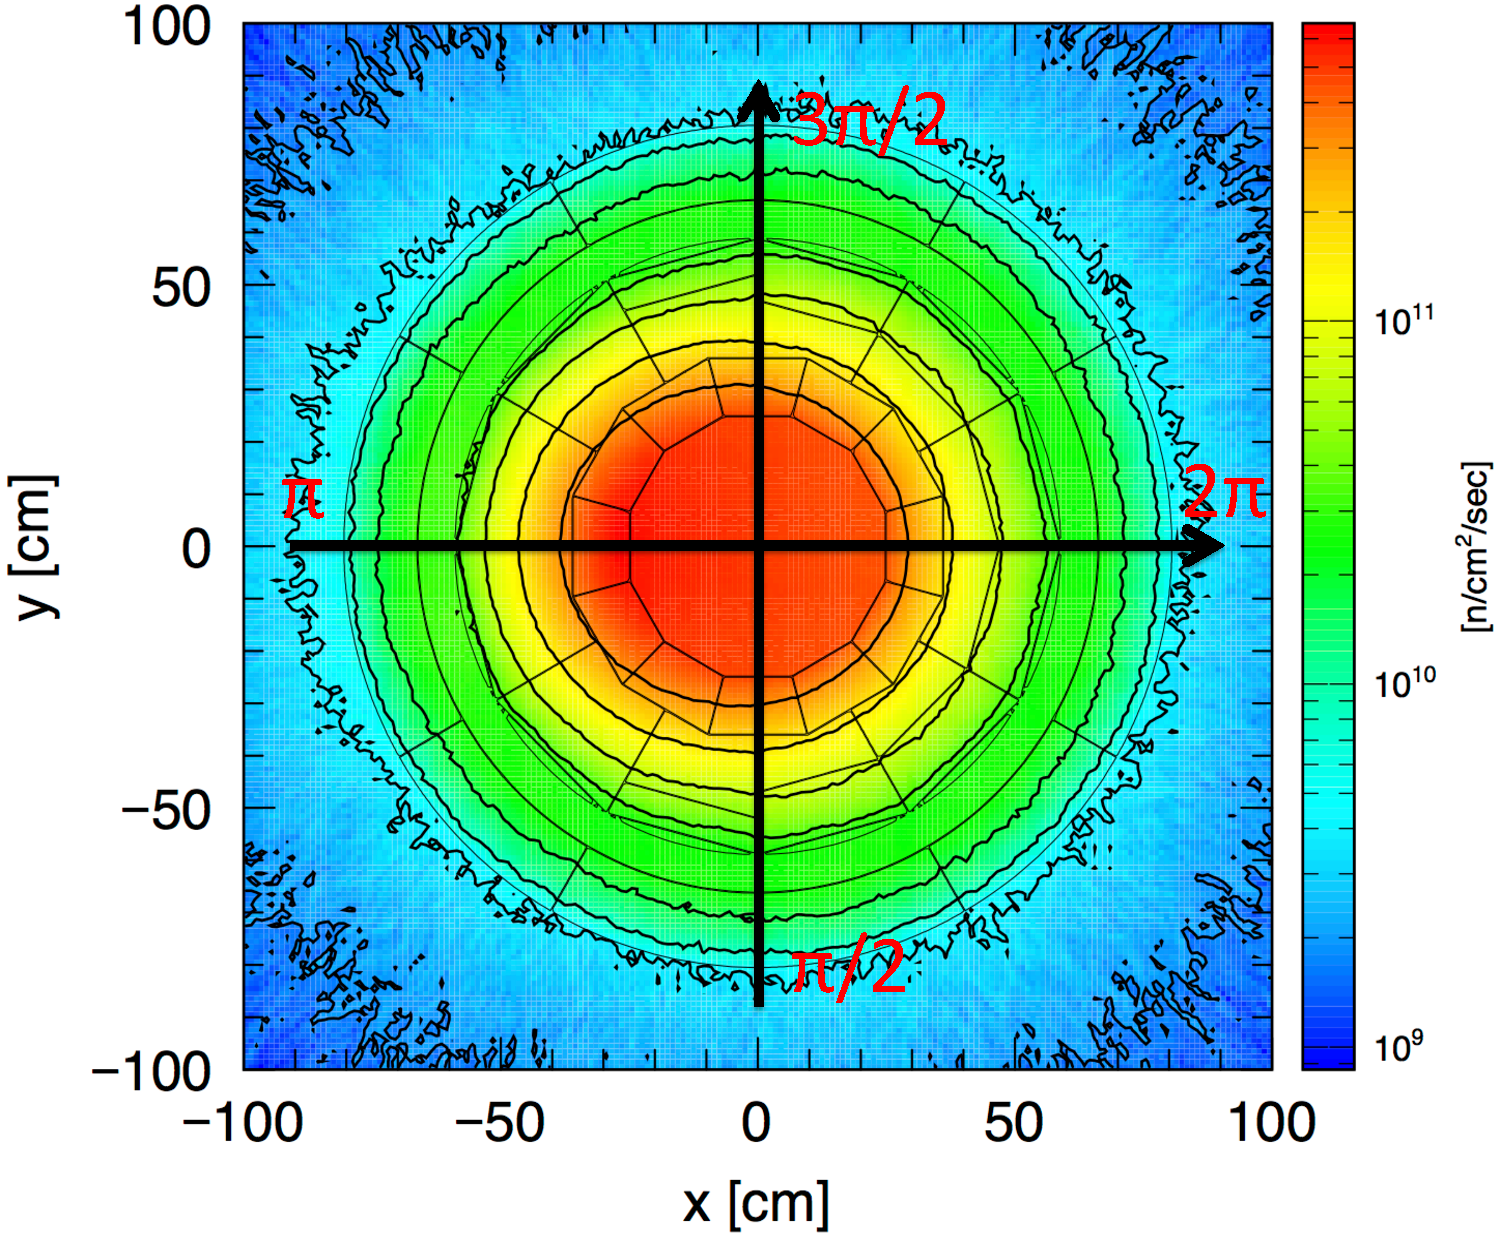
\includegraphics[scale=0.3]{chapter3/fig/shieldflux.pdf}
  \end{subfigure}
  \caption{The concept of COMET radiation shield. It consists of tungsten alloy, stainless steel and copper. Tungsten ally and stainless steel are employed on the high and low radiation side respectively. On the downstream of target, copper is used. Right figure shows the distribution of neutron from x-y view. Azimuthal angle is also defined in here. The peak of neutron flux is located at 180 degree of CS coils.}
  \label{2shieldgeo}
 \end{figure}
\begin{table}[H]
 \centering
 \begin{tabular}{cc} \hline \hline
  Composition [wt.\%] & Ni: 3.0$_{\pm 0.25}$; Cu: 2.0$_{\pm 0.25}$; W: 95.0$_{\pm 0.5}$ \\
  Density [g/cm$^3$] & 18.0$_{\pm 0.2}$ \\
  Hardness & HV 320$_{\pm 50}$ \\
  Tensile strength & 620 MPa \\
  Offset yield strength & 500 MPa \\
  Elastic modulus & 310 GPa \\
  Thermal conductivity & 104 W/m/K \\
  Thermal expansion coefficient & 5.5$\times$10$^{-6}$ K$^{-1}$ \\ \hline \hline
%  Shielding ability & 47\% ($^{60}$Co radiation source) \\
 \end{tabular}
 \caption{Material property of tungsten alloy (AN-1800).}
 \label{alloy}
\end{table}
As shown in figure~\ref{2shieldgeo}, the radiation shield is designed which consists of tungsten alloy, copper and stainless steel.
The DPA, neutron fluence and heat load of several shielding design concepts along azimuthal direction is compared in figure~\ref{2dpa} and \ref{2flux}.
Details of several shielding designs are listed as follows.
 \begin{figure}[H]
  \begin{subfigure}{0.3\textwidth}
   \centering
   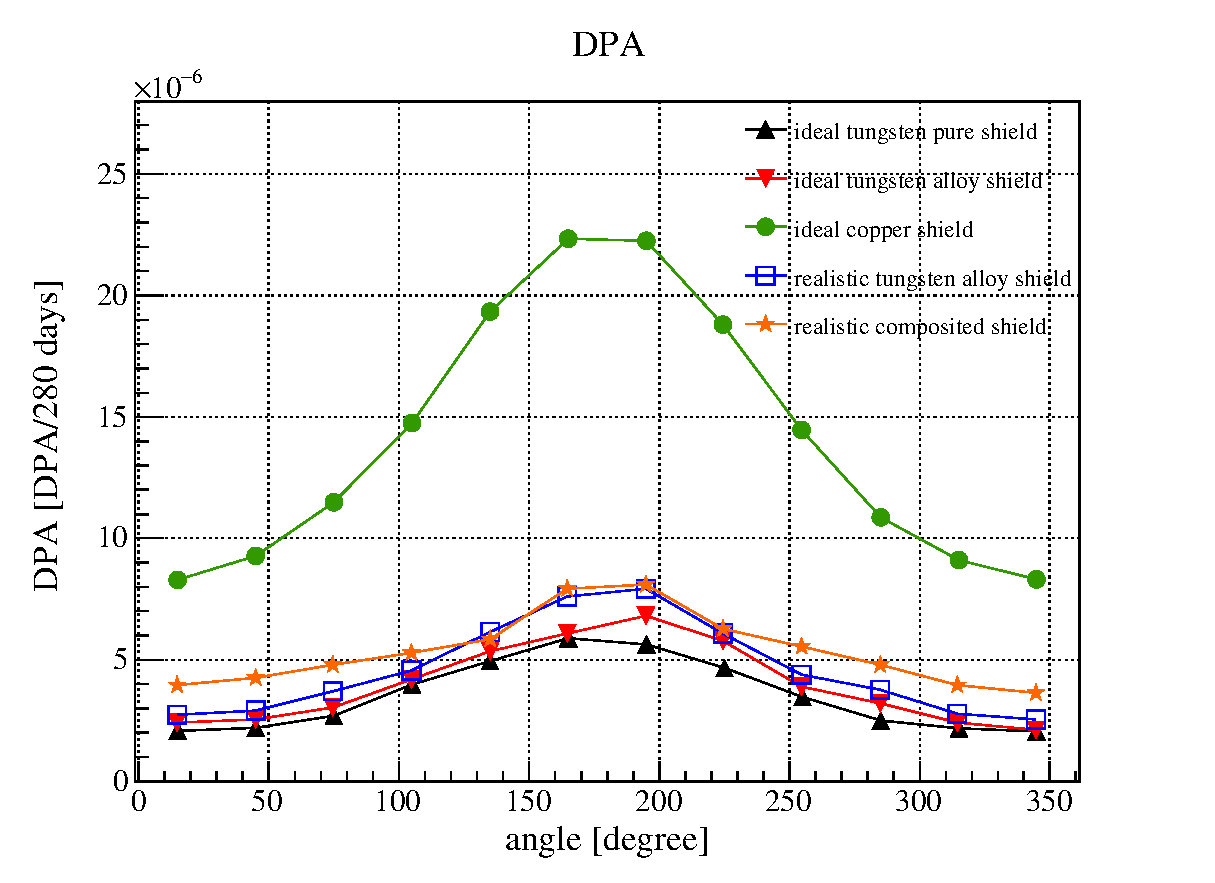
\includegraphics[scale=0.43]{chapter3/fig/dpa.eps}
  \end{subfigure}
  \hspace{0.2\textwidth}
  \begin{subfigure}{0.3\textwidth}
   \centering
   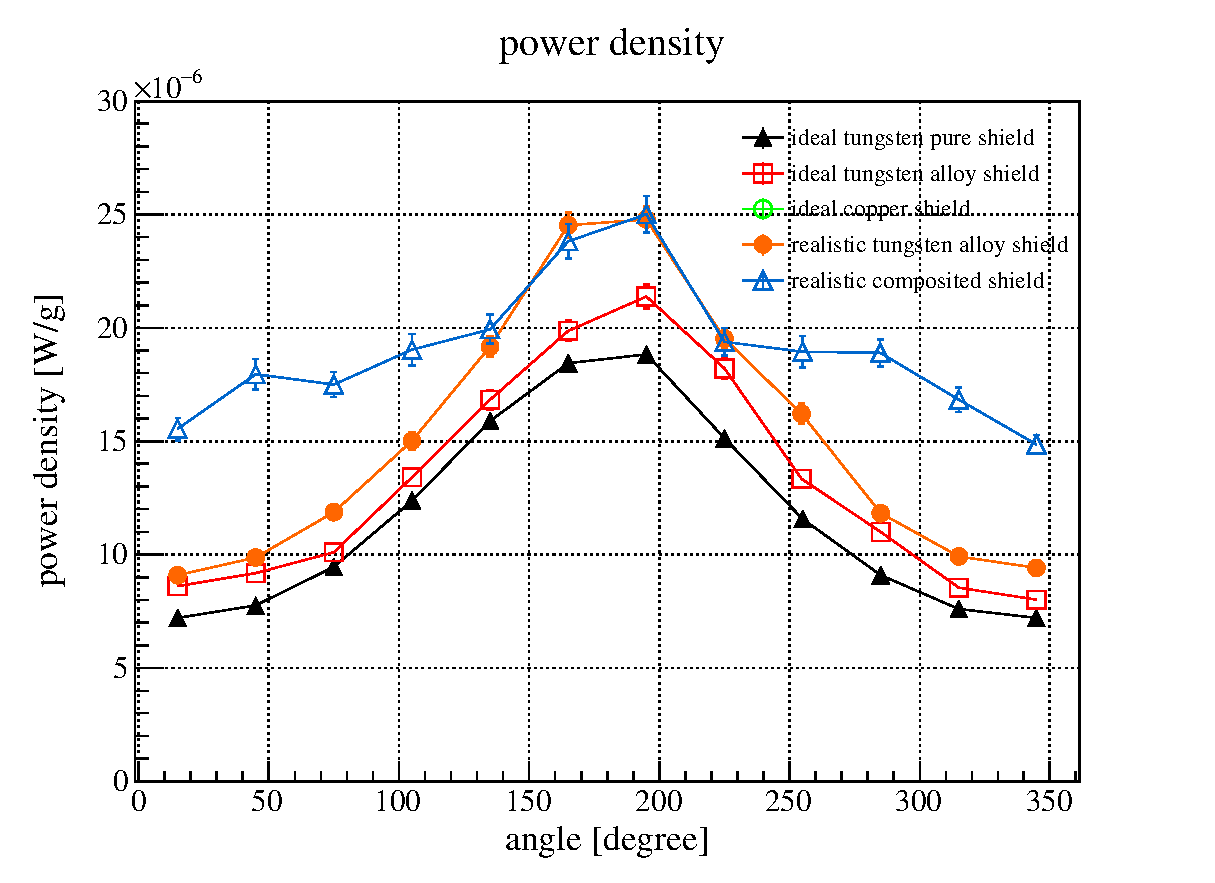
\includegraphics[scale=0.43]{chapter3/fig/shieldheat.eps}
  \end{subfigure}
  \caption{Compared the azimuthal DPA and energy deposition of middel part of CS1 coil in different verion of shielding design. The long CS1 coil is cut to 3 parts along the z axis and 12 parts along the azimuthal axis.}
  \label{2dpa}
 \end{figure}
\begin{itemize}
 \setlength{\itemsep}{-5pt}
 \item Ideal pure tungsten shield: made of pure tungsten with a cylindrical shape.
 \item Ideal tungsten alloy shield: made of tungsten alloy with a cylindrical shape.
 \item Ideal copper shield: made of copper with a cylindrical shape.
 \item Realistic tungsten alloy shield: made of tungsten alloy with a polygonal shape.
 \item Realistic composited shield: made of tungsten alloy, copper and stainless steel with a polygonal shape.
\end{itemize}

After these comparisons, we come out the conclusion
\begin{itemize}
 \setlength{\itemsep}{-5pt}
 \item The maximum DPA of CS1 coils increases over 4 times when the pure tungsten is replaced by copper.
 \item Compared with tungsten alloy, pure tungsten has stronger shielding ability.
 \item Shielding ability of cylindrical shape is stronger than polygonal shape.
 \item The peak of DPA, heat load and neutron fluence is same between composited shield and tungsten alloy shield.
\end{itemize}
The details of shielding design is listed in table~\ref{hrsdet}.
 \begin{figure}[H]
  \centering
  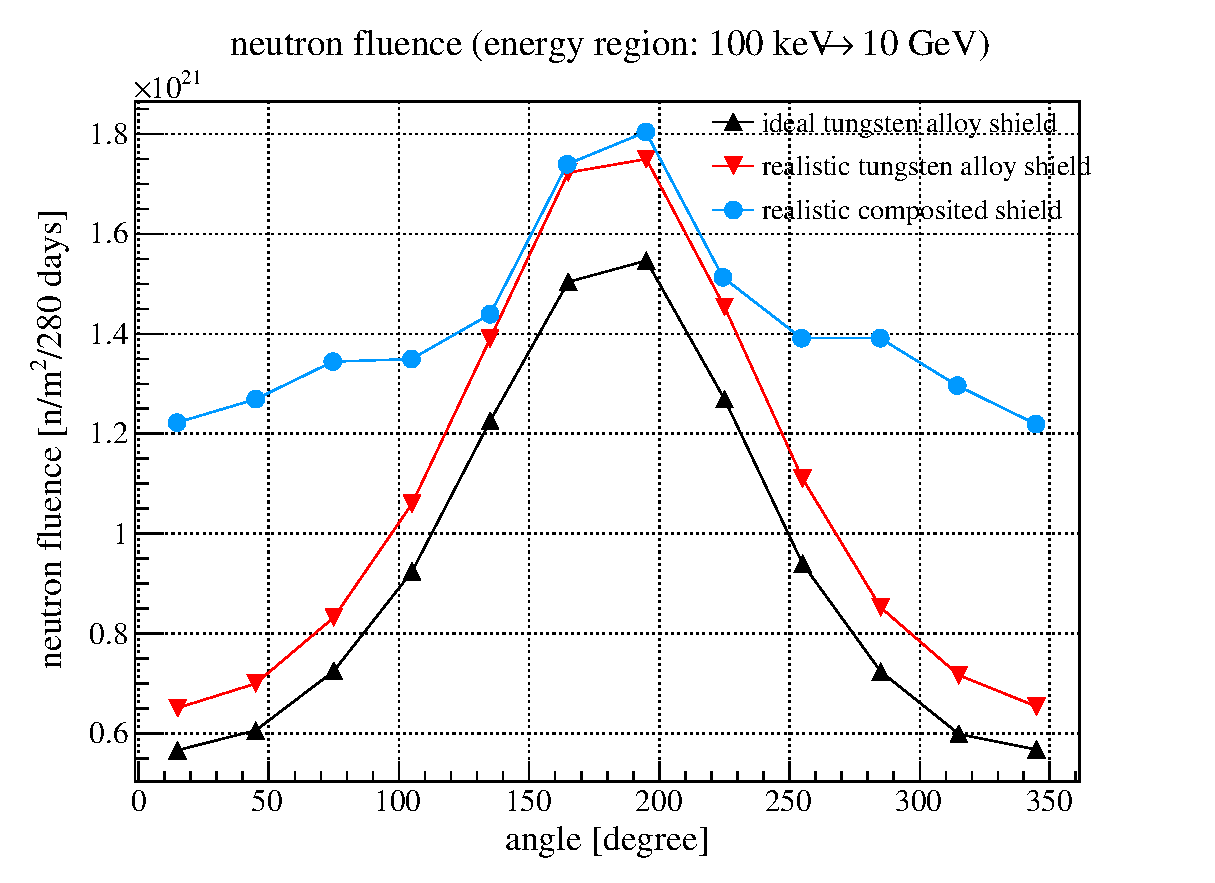
\includegraphics[scale=0.43]{chapter3/fig/fluence}
  \caption{High energy neutron (E $\geq$ 0.1 MeV) along the azimuthal direction of CS1 coils.}
  \label{2flux}
 \end{figure}
\begin{table}[H]
 \centering
 \begin{tabular}{ccc} \hline \hline
  CS1 & Composited shield & Pure tungsten shield \\ \hline
  peak neutron fluence [n/m$^2$/280 days] & 2.35$\times$10$^{21}$ & 2.26$\times$10$^{21}$ \\
  peak power density [W/g] & 2.50$\times$10$^{-5}$ & 2.40$\times$10$^{-5}$ \\
  power [W] & 57.5 & 36.6 \\
  peak dose [MGy/280 days] & 0.79 & 0.76 \\
  peak DPA [DPA/280 days] & 1.05$\times$10$^{-5}$ & 0.98$\times$10$^{-5}$ \\
  tungsten mass [t] & 15.6 & 28 \\ \hline \hline
 \end{tabular}
 \caption{Details of the shielding design. CS1 is cut to 3 parts along the z axis, 12 parts along the azimuthal direction.}
 \label{hrsdet}
\end{table}

As for the muon yield, it does not depend on the material of radiation but the backward radius of shield.
Figure~\ref{radius} shows that the muon and pion yield increases about 9\% after the radius is changed from 36 cm to 50 cm.
\begin{figure}[H]
 \centering
 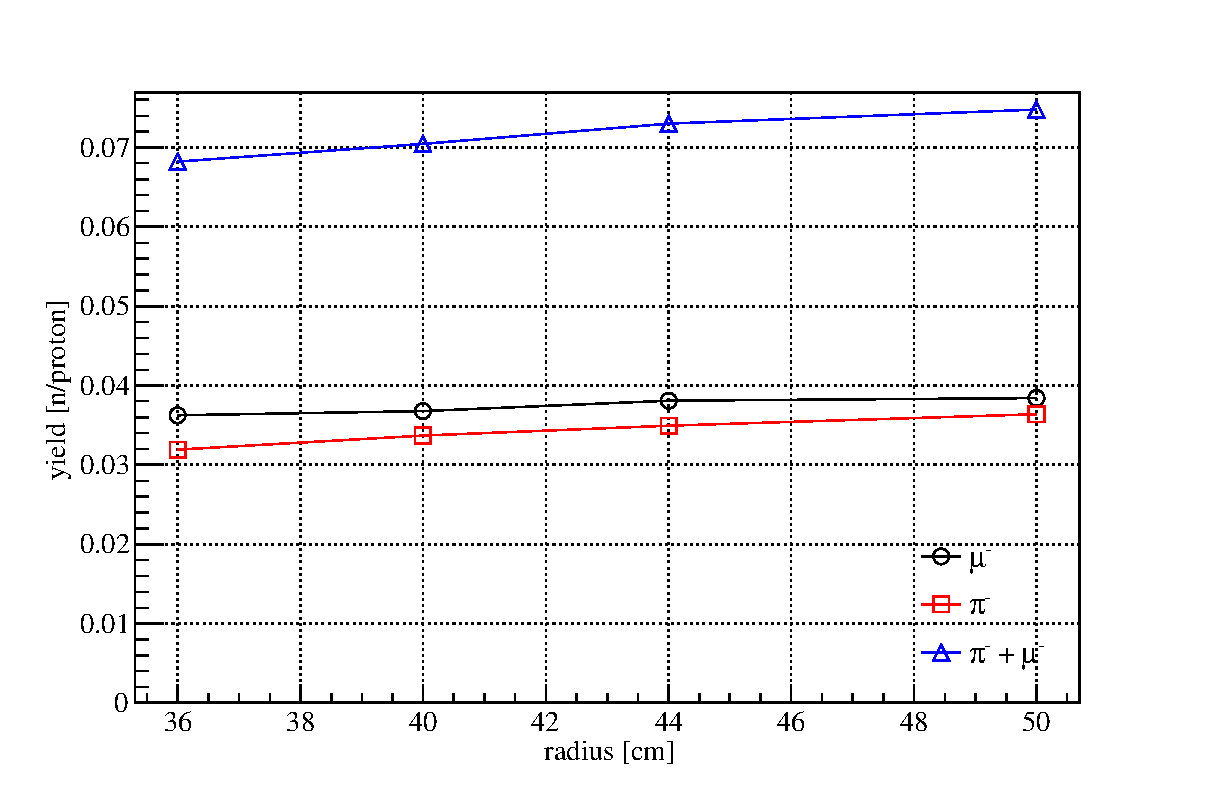
\includegraphics[scale=0.43]{chapter3/fig/muon}
 \caption{A relation of muon and pion yield with shielding backward radius. Current shielding backward radius is 36 cm. Black line: $\mu^-$, red line: $\pi^-$, blue line: $\mu^- + \pi^-$.}
 \label{radius}
\end{figure}

